% -*-coding: utf-8;-*-
%%%%%%%%%%%%%%%%%%%%%%%%%%%%%%%%%%%%%%%%%%%%%%%%%%%%%%%%%%%%%%%%%%%%%%%%%%%%%%
% Главный файл
\documentclass[12pt]{rusthesis}
% do not use [draft] otherwise all PS graphics will disappear
\usepackage[T2A]{fontenc}
\usepackage[utf8]{inputenc}
\usepackage{graphicx}
\usepackage{latexcad}
\usepackage{amsmath}
\usepackage{amssymb}
\usepackage{eepic}
\usepackage{epsfig}
\usepackage{pgf}
\usepackage{tikz}
\usepackage{pstricks}
\bibliographystyle{plain}

\language=4

% My macros
\newcommand\tablref[1]{\cyrt\cyra\cyrb\cyrl.~\ref{#1}}
\newcommand\figref[1]{\cyrr\cyri\cyrs.~\ref{#1}}
\newcommand\pgref[1]{\cyrs.~\pageref{#1}}
%\newcommand\eqref[1]{(\ref{#1})}

\renewcommand{\tan}{\mathop{\rm tg}}
\renewcommand{\arctan}{\mathop{\rm arctg}}
\renewcommand{\tanh}{\mathop{\rm th}}
\newcommand{\DEF}{\mathrel{\mathop=^{\rm def}}}
\newcommand{\MSE}{\overline{\varepsilon^2}}
\newcommand{\hatMSE}{\overline{\hat{\varepsilon}^2}}
\newcommand{\MSEmin}{\overline{\varepsilon^2}_{\rm min}}
\newcommand{\dt}{\Delta t}
\newcommand{\NN}{\mathcal{N}}
\newcommand{\Emax}{|e|_{max}}

% Activation function
\newcommand{\fa}{\phi}

% Gauss Distribution parameters
\newcommand{\GaDi}[2]{$(#1;#2)$}

% Позволить переносы двух последних букв слова
\righthyphenmin=2

% Дополнительные переносы
\hyphenation{ошиб-ки обыч-но сис-тем не-по-сред-ствен-но-го
ус-пеш-но раз-бро-са раз-брос ав-то-рег-рес-сии од-но-вре-мен-но
не-чет-ко-ло-ги-че-ский на-уч-но-ис-сле-до-ва-тель-ских
back-pro-pa-ga-tion out-put}

% Нумерация совсем мелких пунктов
\newcounter{subbbcounter}[subsubsection]
\renewcommand{\thesubbbcounter}{%
\arabic{section}.\arabic{subsection}.\arabic{subsubsection}.%
\arabic{subbbcounter}}
\newcommand{\subbbsection}[1]{\par\bigskip\noindent%
\refstepcounter{subbbcounter}%
{\bf\thesubbbcounter.\quad#1}\nopagebreak\smallskip\par}

% Выводы
%\makeatletter
%\newcommand{\l@conclusion}[2]{\noindent\textbf{#1\hfill #2}}
%\newcommand{\conclusion}[1]{\section*{#1}%
%\addcontentsline{toc}{conclusion}{#1}}
%\makeatother

% Russian document tuning in encoding independent format

\renewcommand\contentsname{\CYRO\cyrg\cyrl\cyra\cyrv\cyrl\cyre\cyrn\cyri\cyre}
\renewcommand\listfigurename{\CYRS\cyrp\cyri\cyrs\cyro\cyrk\
  \cyri\cyrl\cyrl\cyryu\cyrs\cyrt\cyrr\cyra\cyrc\cyri\cyrishrt}
\renewcommand\listtablename{\CYRS\cyrp\cyri\cyrs\cyro\cyrk\
  \cyrt\cyra\cyrb\cyrl\cyri\cyrc}
\renewcommand\refname{\CYRL\cyri\cyrt\cyre\cyrr\cyra\cyrt\cyru\cyrr\cyra}
\renewcommand\indexname{\CYRP\cyrr\cyre\cyrd\cyre\cyrt\cyrn\cyrery\cyrishrt\
  \cyru\cyrk\cyra\cyrz\cyra\cyrt\cyre\cyrl\cyrsftsn}
\renewcommand\figurename{\CYRR\cyri\cyrs.}
\renewcommand\tablename{\CYRT\cyra\cyrb\cyrl\cyri\cyrc\cyra}
%\renewcommand\chaptername{\CYRG\cyrl\cyra\cyrv\cyra}
\renewcommand\partname{\CYRCH\cyra\cyrs\cyrt\cyrsftsn}
\renewcommand\appendixname{\CYRP\cyrr\cyri\cyrl\cyro\cyrzh\cyre\cyrn\cyri\cyre}
\renewcommand\abstractname{\CYRA\cyrn\cyrn\cyro\cyrt\cyra\cyrc\cyri\cyrya}
\def\today{\number\day\space\ifcase\month\or
  \CYRYA\cyrn\cyrv\cyra\cyrr\cyrya\or \CYRF\cyre\cyrv\cyrr\cyra\cyrl\cyrya\or
  \CYRM\cyra\cyrr\cyrt\cyra\or \CYRA\cyrp\cyrr\cyre\cyrl\cyrya\or \CYRM\cyra\or
  \CYRI\cyryu\cyrn\cyrn\cyrya\or \CYRI\cyryu\cyrl\cyrya\or
  \CYRA\cyrv\cyrg\cyru\cyrs\cyrt\cyra\or \CYRS\cyre\cyrn\cyrt\cyrya\cyrb\cyrb\cyrya\or
  \CYRO\cyrk\cyrt\cyrya\cyrb\cyrr\cyrya\or \CYRN\cyro\cyrya\cyrb\cyrr\cyrya\or
  \CYRD\cyre\cyrk\cyra\cyrb\cyrr\cyrya\fi\space\number\year\space\cyrg.}

%\renewcommand\contentsname{\CYRO\cyrg\cyrl\cyra\cyrv\cyrl\cyre\cyrn\cyri\cyre}
%\renewcommand\listfigurename{\CYRS\cyrp\cyri\cyrs\cyro\cyrk\ \cyrr\cyri\cyrs\cyru\cyrn\cyrk\cyro\cyrv}
%\renewcommand\listtablename{\CYRS\cyrp\cyri\cyrs\cyro\cyrk\ \cyrt\cyra\cyrb\cyrl\cyri\cyrc}
%\renewcommand\bibname{\CYRS\cyrp\cyri\cyrs\cyro\cyrk\ \cyrt\cyra\cyrb\cyrl\cyri\cyrc}
%\renewcommand\indexname{\CYRS\cyrp\cyri\cyrs\cyro\cyrk\ \cyrl\cyri\cyrt\cyre\cyrr\cyra\cyrt\cyru\cyrr\cyrery}
%\renewcommand\figurename{\CYRI\cyrn\cyrd\cyre\cyrk\cyrs\ \CYRR\cyri\cyrs\cyru\cyrn\cyro\cyrk}
%\renewcommand\tablename{\CYRT\cyra\cyrb\cyrl\cyri\cyrc\cyra}
%\renewcommand\partname{\CYRCH\cyra\cyrs\cyrt\cyrsftsn}
%\renewcommand\chaptername{\CYRG\cyrl\cyra\cyrv\cyra}
%\renewcommand\appendixname{\CYRP\cyrr\cyri\cyrl\cyro\cyrzh\cyre\cyrn\cyri\cyre}

% end of file

%%%%%%%%%%%%%%%%%%%%%%%%%%%%%%%%%%%%%%%%%%%%%%%%%%%%%%%%%%%%%%%%%%%%%%%%
% Make section and{sub}section number be with final dot in section title
% and in table of contents but not in \ref.  Autoindent in paragraph
% just after section head.
% Part of latex.ltx is used for this task.  Lines which marked by
% %! . after section number
% are changed comparing with original code.
%
% Usage:
% %%%%%%%%%%%%%%%%%%%%%%%%%%%%%%%%%%%%%%%%%%%%%%%%%%%%%%%%%%%%%%%%%%%%%%%%
% Make section and{sub}section number be with final dot in section title
% and in table of contents but not in \ref.  Autoindent in paragraph
% just after section head.
% Part of latex.ltx is used for this task.  Lines which marked by
% %! . after section number
% are changed comparing with original code.
%
% Usage:
% %%%%%%%%%%%%%%%%%%%%%%%%%%%%%%%%%%%%%%%%%%%%%%%%%%%%%%%%%%%%%%%%%%%%%%%%
% Make section and{sub}section number be with final dot in section title
% and in table of contents but not in \ref.  Autoindent in paragraph
% just after section head.
% Part of latex.ltx is used for this task.  Lines which marked by
% %! . after section number
% are changed comparing with original code.
%
% Usage:
% \input{RusStyle.tex}
% in preambule
%%%%%%%%%%%%%%%%%%%%%%%%%%%%%%%%%%%%%%%%%%%%%%%%%%%%%%%%%%%%%%%%%%%%%%%%
\makeatletter%
\renewcommand\section{\@startsection {section}{1}{\z@}%
                                     {3.5ex \@plus 1ex \@minus .2ex}%
                                     {2.3ex \@plus.2ex}%
                                     {\normalfont\Large\bfseries}}
\renewcommand\subsection{\@startsection{subsection}{2}{\z@}%
                                       {3.25ex\@plus 1ex \@minus .2ex}%
                                       {1.5ex \@plus .2ex}%
                                       {\normalfont\large\bfseries}}
\renewcommand\subsubsection{\@startsection{subsubsection}{3}{\z@}%
                                          {3.25ex\@plus 1ex \@minus .2ex}%
                                          {1.5ex \@plus .2ex}%
                                          {\normalfont\normalsize\bfseries}}
\def\@seccntformat#1{\csname the#1\endcsname.\quad}%! . after section number
\def\@sect#1#2#3#4#5#6[#7]#8{%
  \ifnum #2>\c@secnumdepth
    \let\@svsec\@empty
  \else
    \refstepcounter{#1}%
    \protected@edef\@svsec{\@seccntformat{#1}\relax}%
  \fi
  \@tempskipa #5\relax
  \ifdim \@tempskipa>\z@
    \begingroup
      #6{%
        \@hangfrom{\hskip #3\relax\@svsec}%!
          \interlinepenalty \@M #8\@@par}%
    \endgroup
    \csname #1mark\endcsname{#7}%
    \addcontentsline{toc}{#1}{%
      \ifnum #2>\c@secnumdepth \else
        \protect\numberline{\csname the#1\endcsname.}%! . after section number
      \fi
      #7}%
  \else
    \def\@svsechd{%
      #6{\hskip #3\relax
      \@svsec #8}%
      \csname #1mark\endcsname{#7}%
      \addcontentsline{toc}{#1}{%
        \ifnum #2>\c@secnumdepth \else
          \protect\numberline{\csname the#1\endcsname.}%! . after section number
        \fi
        #7}}%
  \fi
  \@xsect{#5}}
\makeatother%

% in preambule
%%%%%%%%%%%%%%%%%%%%%%%%%%%%%%%%%%%%%%%%%%%%%%%%%%%%%%%%%%%%%%%%%%%%%%%%
\makeatletter%
\renewcommand\section{\@startsection {section}{1}{\z@}%
                                     {3.5ex \@plus 1ex \@minus .2ex}%
                                     {2.3ex \@plus.2ex}%
                                     {\normalfont\Large\bfseries}}
\renewcommand\subsection{\@startsection{subsection}{2}{\z@}%
                                       {3.25ex\@plus 1ex \@minus .2ex}%
                                       {1.5ex \@plus .2ex}%
                                       {\normalfont\large\bfseries}}
\renewcommand\subsubsection{\@startsection{subsubsection}{3}{\z@}%
                                          {3.25ex\@plus 1ex \@minus .2ex}%
                                          {1.5ex \@plus .2ex}%
                                          {\normalfont\normalsize\bfseries}}
\def\@seccntformat#1{\csname the#1\endcsname.\quad}%! . after section number
\def\@sect#1#2#3#4#5#6[#7]#8{%
  \ifnum #2>\c@secnumdepth
    \let\@svsec\@empty
  \else
    \refstepcounter{#1}%
    \protected@edef\@svsec{\@seccntformat{#1}\relax}%
  \fi
  \@tempskipa #5\relax
  \ifdim \@tempskipa>\z@
    \begingroup
      #6{%
        \@hangfrom{\hskip #3\relax\@svsec}%!
          \interlinepenalty \@M #8\@@par}%
    \endgroup
    \csname #1mark\endcsname{#7}%
    \addcontentsline{toc}{#1}{%
      \ifnum #2>\c@secnumdepth \else
        \protect\numberline{\csname the#1\endcsname.}%! . after section number
      \fi
      #7}%
  \else
    \def\@svsechd{%
      #6{\hskip #3\relax
      \@svsec #8}%
      \csname #1mark\endcsname{#7}%
      \addcontentsline{toc}{#1}{%
        \ifnum #2>\c@secnumdepth \else
          \protect\numberline{\csname the#1\endcsname.}%! . after section number
        \fi
        #7}}%
  \fi
  \@xsect{#5}}
\makeatother%

% in preambule
%%%%%%%%%%%%%%%%%%%%%%%%%%%%%%%%%%%%%%%%%%%%%%%%%%%%%%%%%%%%%%%%%%%%%%%%
\makeatletter%
\renewcommand\section{\@startsection {section}{1}{\z@}%
                                     {3.5ex \@plus 1ex \@minus .2ex}%
                                     {2.3ex \@plus.2ex}%
                                     {\normalfont\Large\bfseries}}
\renewcommand\subsection{\@startsection{subsection}{2}{\z@}%
                                       {3.25ex\@plus 1ex \@minus .2ex}%
                                       {1.5ex \@plus .2ex}%
                                       {\normalfont\large\bfseries}}
\renewcommand\subsubsection{\@startsection{subsubsection}{3}{\z@}%
                                          {3.25ex\@plus 1ex \@minus .2ex}%
                                          {1.5ex \@plus .2ex}%
                                          {\normalfont\normalsize\bfseries}}
\def\@seccntformat#1{\csname the#1\endcsname.\quad}%! . after section number
\def\@sect#1#2#3#4#5#6[#7]#8{%
  \ifnum #2>\c@secnumdepth
    \let\@svsec\@empty
  \else
    \refstepcounter{#1}%
    \protected@edef\@svsec{\@seccntformat{#1}\relax}%
  \fi
  \@tempskipa #5\relax
  \ifdim \@tempskipa>\z@
    \begingroup
      #6{%
        \@hangfrom{\hskip #3\relax\@svsec}%!
          \interlinepenalty \@M #8\@@par}%
    \endgroup
    \csname #1mark\endcsname{#7}%
    \addcontentsline{toc}{#1}{%
      \ifnum #2>\c@secnumdepth \else
        \protect\numberline{\csname the#1\endcsname.}%! . after section number
      \fi
      #7}%
  \else
    \def\@svsechd{%
      #6{\hskip #3\relax
      \@svsec #8}%
      \csname #1mark\endcsname{#7}%
      \addcontentsline{toc}{#1}{%
        \ifnum #2>\c@secnumdepth \else
          \protect\numberline{\csname the#1\endcsname.}%! . after section number
        \fi
        #7}}%
  \fi
  \@xsect{#5}}
\makeatother%


% TeXdraw toolbox macros, useful for extended TeXdraw commands

% $Id: txdtools.tex,v 1.1 2001-05-02 16:08:46 vlad Exp $

%   Copyright (C) 1991,1992  Peter Kabal

% The routines in this file are provided free of charge without
% warranty of any kind.  Note that the TeXdraw routines are copyrighted.
% They may be distributed freely provided that the recipients also
% acquire the right to distribute them freely.  The notices to this
% effect must be preserved when the files are distributed.

%  Peter Kabal
%  Department of Electrical Engineering
%  McGill University
%  3480 University
%  Montreal, Quebec
%  Canada  H3A 2A7

%  kabal@TSP.EE.McGill.CA
 
% ===============================================================

% These macros use temporary count registers defined by TeXdraw
%  \t@counta     \t@pixa
%  \t@countb     \t@pixb
%  \t@countc     \t@pixc
%                \t@pixd

\chardef\catamp=\the\catcode`\@
\catcode`\@=11


% ===== Real arithmetic
% Real addition
%  #1  - summand
%  #2  - summand
%  #3  - macro name to capture the real result
\def\realadd #1#2#3{\dimen0=#1pt
                    \dimen2=#2pt
                    \advance \dimen0 by \dimen2
                    \edef #3{\expandafter\c@lean\the\dimen0}}

% Real division
%  #1 - numerator
%  #2 - denominator (divisor)
%  #3 - macro name to capture the real result
\def\realdiv #1#2#3{\dimen0=#1pt
                    \t@counta=\dimen0
                    \dimen0=#2pt
                    \t@countb=\dimen0
                    \intdiv \t@counta \t@countb #3}

% ===== Integer arithmetic

% Length of the hypotenuse
% Find the length of a vector, lenhyp = sqrt(dx*dx + dy*dy)
%  #1 - integer value, dx
%  #2 - integer value, dy
%  #3 - count register to capture the integer value
\def\lenhyp #1#2#3{\t@counta=#1%
                   \multiply \t@counta by \t@counta
                   \t@countb=#2%
                   \multiply \t@countb by \t@countb
                   \advance \t@counta by \t@countb
                   \sqrtnum \t@counta #3}

% Square root of an integer
% Newton-Raphson iteration to find the square root, integer argument
% Let the current estimate of the square root of x be b(k).
% Form an error function, e(k)=b(k)*b(k)-x. Follow the gradient of the
% error to calculate the next guess,
%
%    e(k) - 0     d e(k)                          b(k) + x/b(k)
%   ----------  = ------  = 2*b(k)  ==>  b(k+1) = -------------
%   b(k)-b(k+1)   d b(k)                               2
%
% Note this iteration does not work for x=0, since the guess is then b(k)=0.
% Rename the count registers to have more suggestive names
\let\bk=\t@counta
\let\bn=\t@countb
\let\xval=\t@countc
\def\sqrtnum #1#2{\xval=#1%
                  \bk=\xval
                  \loop
                    \bn=\xval
                    \divide \bn by \bk
                    \advance \bn by \bk
                    \advance \bn by 1            % rounding
                    \divide \bn by 2
                  \ifnum \bn < \bk
                    \bk=\bn
                  \repeat
                  #2=\bn}

% ===== Coordinate macros

% Return the coordinates of the current position
%  #1 - macro name to capture the x-coordinate
%  #2 - macro name to capture the y-coordinate
\def\currentpos #1#2{\t@pixa=\x@pix
                     \advance \t@pixa by -\x@segoffpix
                     \pixtocoord \t@pixa #1
                     \t@pixa=\y@pix
                     \advance \t@pixa by -\y@segoffpix
                     \pixtocoord \t@pixa #2}

% Length of a vector
% Find the length of the vector between coordinate (#1 #2) and
% coordiante (#3 #4). The length is expressed relative to the
% current scaling.
%  (#1 #2) - vector start coordinates
%  (#3 #4) - vector end coordinates
%  #5 - macro name to receive the length
\def\vectlen (#1 #2)(#3 #4)#5{\getpos (#1 #2)\x@arga\y@arga
                              \getpos (#3 #4)\x@argb\y@argb
                              \coordtopix \x@arga \t@pixa
                              \coordtopix \x@argb \t@pixb
                              \advance \t@pixb by -\t@pixa
                              \coordtopix \y@arga \t@pixc
                              \coordtopix \y@argb \t@pixd
                              \advance \t@pixd by -\t@pixc
                              \lenhyp \t@pixb \t@pixd \t@pixc
                              \pixtocoord \t@pixc #5}

% Cossine and sine
% Find the cosine and sine of the angle of a vector directed from
% the coordinate (#1 #2) to the coordinate (#3 #4).
%  (#1 #2) - start coordinates
%  (#3 #4) - end coordinates
%  #5 - macro name to receive the cosine of the angle
%  #6 - macro name to receive the sine of the angle
\def\cossin (#1 #2)(#3 #4)#5#6{\getpos (#1 #2)\x@arga\y@arga
                               \getpos (#3 #4)\x@argb\y@argb
                               \coordtopix \x@arga \t@pixa
                               \coordtopix \x@argb \t@pixb
                               \advance \t@pixb by -\t@pixa
                               \coordtopix \y@arga \t@pixc
                               \coordtopix \y@argb \t@pixd
                               \advance \t@pixd by -\t@pixc
                               \lenhyp \t@pixb \t@pixd \t@pixc
                               \intdiv \t@pixb\t@pixc #5%
                               \intdiv \t@pixd\t@pixc #6}

\catcode`\@=\catamp

% Block diagrams in TeXdraw

% $Id: blockdiagram.tex,v 1.1 2001-05-02 16:08:45 vlad Exp $

%   Copyright (C) 1993  Peter Kabal

% The routines in this file are provided free of charge without
% warranty of any kind.  Note that the TeXdraw routines are copyrighted.
% They may be distributed freely provided that the recipients also
% acquire the right to distribute them freely.  The notices to this
% effect must be preserved when the files are distributed.

%  Peter Kabal
%  Department of Electrical Engineering
%  McGill University
%  3480 University
%  Montreal, Quebec
%  Canada  H3A 2A7

%  kabal@TSP.EE.McGill.CA
 
% ===============================================================

\input txdtools

% size of sum and product circles
\def\cradius{0.08}

% \bdot
% big dot
\def\bdot{\fcir f:0 r:0.02 }

% centred, stacked items
\def\hcp#1{$\vcenter{\halign{\hss ##\hss\cr #1\crcr}}$}

% left justified, stacked items
\def\hlp#1{$\vcenter{\halign{##\hss\cr #1\crcr}}$}

% right justified, stacked items
\def\hrp#1{$\vcenter{\halign{\hss ##\cr #1\crcr}}$}

% signal labels - Top text, Bottom text, Left text, Right text,
% and Center text
\def\Ttext#1{\bsegment
               \textref h:C v:B  \htext (0 +0.06){\hcp{#1}}
             \esegment}
\def\Btext#1{\bsegment
               \textref h:C v:T  \htext (0 -0.06){\hcp{#1}}
             \esegment}
\def\Ltext#1{\bsegment
               \textref h:R v:C  \htext (-0.06 0){\hrp{#1}}
             \esegment}
\def\Rtext#1{\bsegment
               \textref h:L v:C  \htext (+0.06 0){\hlp{#1}}
             \esegment}
\def\Ctext#1{\bsegment
               \textref h:C v:C  \htext{\hcp{#1}}
             \esegment}

% ruled box (horizontal) with centered label,
% position set to the end of the box
% \Fbox W H text
\def\Fbox#1#2#3{\bsegment
                  \bsegment
                    \setsegscale 0.5
                    \textref h:C v:C  \htext (#1 0){\hcp{#3}}
                  \esegment
                  \setsegscale 0.5 \lvec (0 #2)
                  \setsegscale 1
                  \rlvec (#1 0) \rlvec (0 -#2) \rlvec (-#1 0) \lvec (0 0)
                  \savepos (#1 0)(*@x *@y)
                \esegment
                \move (*@x *@y)}

% ruled box (vertical) with centered label, position set to the end of the box
% \Gbox W H text
\def\Gbox#1#2#3{\bsegment
                  \bsegment
                    \setsegscale 0.5
                    \textref h:C v:C  \htext (0 #2){\hcp{#3}}
                  \esegment
                  \setsegscale 0.5 \lvec (#1 0)
                  \setsegscale 1
                  \rlvec (0 #2) \rlvec (-#1 0) \rlvec (0 -#2) \lvec (0 0)
                  \savepos (0 #2)(*@x *@y)
                \esegment
                \move (*@x *@y)}

% ruled triangle (horizontal) with centered label,
% position set to the end of the box
% \Ftri W H text
\def\Ftri#1#2#3{\bsegment
                  \bsegment
                    \setsegscale 0.3333
                    \textref h:C v:C  \htext (#1 0){\hcp{#3}}
                  \esegment
                  \bsegment
                    \savepos (#1 0)(*@x *@y)
                  \esegment
                  \setsegscale 0.5 \lvec (0 #2)
                  \setsegscale 1   \lvec (#1 0)
                  \setsegscale 0.5 \lvec (0 -#2) \lvec (0 0)
                \esegment
                \move (*@x *@y)}

% \pluss
% plus sign
\def\pluss {\bsegment
              \setsegscale {\cradius}
              \move (-0.5 0) \lvec (+0.5 0)
              \move (0 -0.5) \lvec (0 +0.5)
            \esegment}

% \minuss
% minus sign
\def\minuss {\bsegment
               \setsegscale {\cradius}
               \move (-0.5 0) \lvec (+0.5 0)
             \esegment}
% \mults
% multiplication sign
\def\mults {\bsegment
              \setsegscale {\cradius}
              \realmult \cradius {0.354} \tmpa
              \move (-0.354 -0.354) \lvec (+0.354 +0.354)
              \move (-0.354 +0.354) \lvec (+0.354 -0.354)
            \esegment}

% \pcir
% circle of given radius with a plus sign
\def\pcir {\lcir r:{\cradius}  \pluss}

% \mcir
% circle of given radius with a multiplication sign
\def\mcir {\lcir r:{\cradius}  \mults}

% \putn, \putnne, etc
% places text at an offset from the center of a circle, with
% the position of the text specified in compass directions
\def\puttext (#1 #2)#3{\bsegment
                         \setsegscale {\cradius}
                         \textref h:C v:C \htext (#1 #2){#3}
                       \esegment}
\def\putn   #1{\puttext ( 0   +2  ){#1}}
\def\putnne #1{\puttext (+1.2 +1.7){#1}}
\def\putene #1{\puttext (+1.7 +1.2){#1}}
\def\putese #1{\puttext (+1.7 -1.2){#1}}
\def\putsse #1{\puttext (+1.2 -1.7){#1}}
\def\puts   #1{\puttext ( 0   -2  ){#1}}
\def\putssw #1{\puttext (-1.2 -1.7){#1}}
\def\putwsw #1{\puttext (-1.7 -1.2){#1}}
\def\putwnw #1{\puttext (-1.7 +1.2){#1}}
\def\putnnw #1{\puttext (-1.2 +1.7){#1}}


% \avectoc
% arrow vector to a circle
\def\avectoc (#1 #2){\currentpos \xa\ya
                     \cossin ({\xa} \ya)(#1 #2)\cosa\sina
                     \savepos (#1 #2)(*@x *@y)%
                     \bsegment
                       \move (*@x *@y)%
                       \setsegscale {\cradius}
                       \rmove ({-\cosa} -\sina)%
                       \savecurrpos (*@x *@y)%
                     \esegment
                     \avec (*@x *@y)%
                     \move (#1 #2)}
% \avecfrc
% arrow vector from a circle
\def\avecfrc (#1 #2){\currentpos \xa\ya
                     \cossin ({\xa} \ya)(#1 #2)\cosa\sina
                     \bsegment
                       \setsegscale {\cradius}
                       \move ({\cosa} \sina)%
                       \savecurrpos (*@x *@y)%
                     \esegment
                     \move (*@x *@y)%
                     \avec (#1 #2)}
% \avecfrctoc
% arrow vector from a circle to a circle
\def\avecfrctoc (#1 #2){\currentpos \xa\ya
                        \cossin ({\xa} \ya)(#1 #2)\cosa\sina
                        \bsegment
                          \setsegscale {\cradius}
                          \move ({\cosa} \sina)%
                          \savecurrpos (*@x *@y)%
                        \esegment
                        \move (*@x *@y)%
                        \avectoc (#1 #2)}
% \lvecfrc
% line vector from a circle
\def\lvecfrc (#1 #2){\currentpos \xa\ya
                     \cossin ({\xa} \ya)(#1 #2)\cosa\sina
                     \bsegment
                       \setsegscale {\cradius}
                       \move ({\cosa} {\sina})%
                       \savecurrpos (*@x *@y)%
                     \esegment
                     \move (*@x *@y)%
                     \lvec (#1 #2)}


% Для макросов texdraw установить умолчательной единицей измерения миллиметры
%texdraw \everytexdraw{\drawdim mm}

\title{Стохастический квазиоптимальный нейросетевой регулятор}

\author{Елисеев Владимир Леонидович}

\begin{document}

% Титульные страницы
%\maketitle

% Оглавление
\setcounter{tocdepth}{4}\tableofcontents
%\newpage

% Введение
\chapter*{Введение}
\addcontentsline{toc}{chapter}{Введение}

%% -*-coding: cp1251;-*-
%%%%%%%%%%%%%%%%%%%%%%%%%%%%%%%%%%%%%%%%%%%%%%%%%%%%%%%%%%%%%%%%%
% ��������

\newcommand{\NumberOfPages}{\pageref{LastPage}}
% -*-coding: cp1251;-*-
%%%%%%%%%%%%%%%%%%%%%%%%%%%%%%%%%%%%%%%%%%%%%%%%%%%%%%%%%%%%%%%%%
% ��������

\paragraph{������������ ������}
����� �� ������ ����������� ������������� ������������� ���������
����� (���) ������� ��������������� ���������� ��������� �����.
�������� ������� ��������� ������������� ������� ��������� �����,
����� ��� ���������� �������� ���������.  ��������� ���� �� ��������
������������ � ������������� ��� ���������� �������������� �
���������� ������������, � �������������� � ������������
����������������� ���������� ������ �����, � ������� ���������� ���
������������� � ���������� ����������� ����������.

��� ��� ������� ���������� ������������� � ������������ ������������
��������� �����, ������������ �� ���������� � �������� ����������, �
����� ������������� � ������� ���������.  � ���� �� ������� � ������
����������������� ���������������� ������-������������� �����������,
�������� ������� ������� � ������������� ������ �������������
����������.

������ �� ������ �������� ������ � ������� ������ ���������� ���
�������������� (�.~�.~��������, �.~�.~�������, �.~�.~�������,
�.~�.~�����������, �.~�.~�������, �.~�.~�������, �.~�.~��������� �
��.), ��� � ����������� ������� (�.~��������, �.~������, �.~������,
�.~�����, �.~�������� � ��.). ��� �� �����, ������ ������� ����
����������� ������������ �����, ���� ������������� �� �������
������������ ����� ���������� �����.  � ���������, ����������� ������,
����������� �������������� ������ ������������� ���������� ��
������������, ���������� ����������� � ���������� ������� ����
���������� ���������.  ��� ����������, � ������� ��������������
������������ � �������� ���������� ��� ������������� ������
��������������������� �������� �������������.  ���������� ���������
�������� ����� �� ������������� ���������� �������������� ��������.
�� ��� ��������������� � ������������� ����������� ��������
������������ �� ������ ������������.

������������� ������ ������� ������������ ����������� � �������
������������ ����� ������������������ ����� � ���������� ���� � �����
����������� ���������, ���������� ��������� ������ � ��������.  �����
���, ����������� ������������ ����������� ������������� �����,
����������� ��������� �������������� ���������� �������
���������������, � ����� ����������� �������������� �������� �������.
������� ��� ������� ����������� �������������� ������ ��������� �����.
� �� �� �����, � ������ ���������� ������� �����, ������� ������������
��������, ����� ��� �������� ��������� ���������� ������������,
����������� ���������� ������������� ���������� ��� ����������
������������ � �������������� �������� ��������, �������������� �
����������� �������������� ������������, ������������ �� �����������
������� ���������� ��������� �����.  ����� ������ ����� ��������� �
������ �������������� ������������ ������������ �������������, �
������������� �������� � ��������� ��������� �� ��������� � ��������
��������.

\paragraph{���� ������������}
����� ��������������� ������ �������� �������� ������� � ����������
������������� ���������� � �������� �� �������������� � �����������
������������ ��������.

% � ���������, �������������� ������ ����������� ������� ������
% ��������� ������ � ����������� ��������� �����, ������� ��������
% ������ �� ��������� ��������� ����, �������������� ������������ �
% ����� ������ ������������� ���������� ��������� ��������
% ������������ ����������� � ������� ���������� � ��� ��� ��� � ������
% ���������� �������, ��� � � �������������� ��������.

\paragraph{������ ������������}
� ������������ � ��������� ����� � ������ ��������������� ������
���������� � �������� ��������� ������:
\begin{enumerate}
\item
����� � ������ ��������� �������� ���������� ��� � ��������
����������, ������������ ������� � ����������� �������.

\item
���������� �������� ������� ������������� ���������� � ������� �, �� �
��� ����������� � ������������� �� �������.

\item
������������ ������������ ������������� ������� ��� ���������� ��� ��
�������� �������� �������������������� ������.

\item 
�������� ������������ ���������� ���������� ��������������� ���������.

\item
���������� ���������� ������������, �������������� �
����������-��������������� ����������� ��� ������� ������������ �����
���������� ��������� ������� � � ������� ��������.
\end{enumerate}

\paragraph{������ ������������}
���������� ���������� ������������ ���������� �� ������������� �������
� ������� ���������� �������, ������ ������������� ��������� ����� �
������ ��������������� ����������, �������������� ����������,
������������� �������������.

\paragraph{������� �������}

\begin{enumerate}
\item 
����������� �������� ������� ������������� ���������� --- ������� �,
�� � ��� �����������, --- ���������� � ���� ����� ��������� ������ �
���������� ����������� ������������ ���, ����������� ������������
��������� �������, ���������� �������� ���, �������������� ������
��������� ���������� �� ������������ ��� ������ �������� ����������.

\item
���������� ������ ���������� � ��������� ������������� ���������� ��
�������� �������� �������������������� ������ � �������������� ���
������������� � ����������� �������� � ����������� ��� ���������
���������� �������� � ������� ����������.

\item
���������� �������� ���������� �������������� �������� �� ������
���������������� ������������� ������������� � ���������������
��������.
\end{enumerate}


\paragraph{�������������� � ������������� ������� ���������, �������
� ������������} �������������� ���������� �������������� �������
������ ������������� ��������� ����� � ������ ���������������
����������, ������������ ������������� ������������� � ����������
������������� �������, ���������� � ���������� �������� � ������
�������� �������������.

\paragraph{������������ ���������� ������}
���������� ������������, ����������� � ��������������� ������, ����
������������ ��� ������� ������������� ��������� ���������� ���������
������� � ���������� �� ��������.  ������������� ������ ���������
����� ������������ ������������ �������� ��� ���������� �������
������� ��������� ��������� � ���������� �����-�����������
���������������� � ������������� ���������� ��� ����������
������������� ������������� ���������� ����������.  ���������
��������� ����� � ������ ������������ ��������� �������������
������������ ������ ����������, ������� ����� �������������� ���
������� � ������������ ������������ ���������� ���������� � ��
��������� � ��������������� ���������.  ������ �������� ��������
�������������, ���������, ����� ����������� ��� ������������� ������ �
����������� ��� ���������� � ������� �������� � �������� ������������
������ ��� ���������� ������������ �����.

\paragraph{���������� �����������}

���������� ������ ���� ������������:
\begin{itemize}
\item
��� ���������� ��������� ������������� ���������� ���������� ���������
������� � ���������� ��������������� ����������� ������������
��. �.~�.~�������;
\item
��� �������� ������-������������� ������������� ��������� �� �����
``��������������� � �� ����������'' � ������������ �����������������
������������ ���.
\end{itemize}

\paragraph{��������� ������} ���������� ������ � �� �������� ���������
������������� �� ���������� � ������������� ������������
``�������������� ���������� � �����, �����������, ���������������� �
�������'' � IT+SE (����-������, 2010~�., 2011~�.), ``��������������
�������� � ����������'' (������, 1999~�., 2000~�.), ``����������
�������� ������ � ������������'' (�����-���������, 2006~�.),
``International Scientific Colloquium'' (��������, ��������, 2000~�.,
2010~�.), �� ��������� ������� ``���������� � �����������''
������������ ����������������� ������������ ���.



\paragraph{����������}
�� ����������� ������������ ������������ 13 �������
����� \cite{el-neurocomp2002,elzenk-extrob2006,elfil-pta99,elfil-modctrl2006,
elfil-vestmei2010,filel-ict2000,filel-ict2003,filelav-ict99,
elfil-iwk2000,filel-iwk2010,el-trainset2010,elfil-labsoft2011,el-nit2011}, � ���
�����, 2 ���������� � ������������� ��������, �������� � ������ ���
��:~\cite{elfil-vestmei2010,elfil-labsoft2011}.

\paragraph{��������� � ����� ������}
%\marginpar{���������!}
��������������� ������ ������� �� ��������, ����� ����, ���������� �
������ ���������� �� 85 ������������, �������� \NumberOfPages\ �������
������, 72 �������, 14 ������.

% Take care of autoreferat!!!
% Number of figures may be counted so:
%  $ grep 'label[{]fig:' *.tex | wc -l
% Number of tables may be counted so:
%  $ grep 'label[{]tabl:' *.tex | wc -l

\paragraph{������� ����� ����}

% ����� 1

� ������ ����� �������� ����� ���������� ��������, � ������� �������
����������� ������� ���������� ��������� ����� � �������� ����������.
������ ������� ������ ������ ������������ ���� ������������.

��������������� �������� ����������� ��������� �����, ����������� �
�������� ����������.  ����������� �� ���������� � ����������
������������� �� ������� ���������� ������������ �������.
������������� ������� � ������������������� ��������� ��������.
������������� �������, ����������� ��� �������������� ��������� ���
������� ���������� ���������� ������.

�� ������ ������� ���������� ������������� �������� ������� ����������
��������� ����� � �������� ����������.  �������� ��������������� �
������������� ��������� ������� � ������� ������������� ����������.
����������� �������� ����� ��������, ����������� ���������������, � ��
��������.  ����� �������� ����� ������� ������������ ������������� �
�� ������������� � �������� �������� �������������.  ���������� �����
���������� ������������ ������� � ���������� ����������� �����������
��� �� ������� � ������������.  � ��������� ������ �������� ������
������� ������������� ���������� ��������� �����.  ���� ��������
��������� ����������, ���������--����������� ����������� ���� ����� �
��������� ������������ ����������.

�������������� �������� ���������� ���������������� �������������
������������ �������� � ������������ �����������, � ����� ���������
������������� ������� ���������.  ������������� ���������� �� ������
��������.  ���������� ���������������� ��������� ��� � ��������
���������������� ��� ����������� ��-�� ������� ������������ ��������
������ ������������, ��� � � ����������� ����������� ����������� �
���� ��������������� ���������� ������ �������, ��� ������
������������� ����������� ����������.

��������������� �������� ������, ����������� ��� �������� ���������
����� � �������� ����������.  ���������� ��������� �� ���������� �
�������� ������� �������������� � ������������� �������������.
�������� ��������������� online-�������, ������������ ��� ������������
������������ ���������� � �������������� �� ���������� � ����� ������
������������� ������ �����.  �������� ����� �� ������������ ����������
������������ ������, ������������ � ���� ����������� ������������� ���
� �������� ��������� ����� � ����� ������������� � ������� ��������.

% ����� 2

�� ������ ����� ������������� ������ ������ ��� ���������� ��
������������ � ������� ������������� ������� ��� ���������� ����������
��� ������� ���������� �� �������� ����������� ��������������������
������ ��������.  ������������ �������� ����� �������� �������
������������� ���������� (��--�), ����� ������� ����� �����������
���������, ���� ��������� ������, ��������, �������� �������� ��������
� ����������������.

����� ��������������� ������ ������ ����������� ��������� ����������.
��� ������������ ���������� ������������ ������ ������ ��� ����������
������������ �������, ���������� ����� ���� � ������������� �������� �
���.  ��������������� ��������������� �������� ����������� �����������
� � ������ ������������ ������������� ���������� �������� ����������
�� ���.

���������� ������������ � ������� ���� �������� �������, �������������
��� ��������� ��������� �������, �� �������� �������� ��--�.
����������� ������ ��������� �������������� �������� ��������,
�������������� �������� ��������������� ������������� ���������� ---
������� ������������� ������������� ������ ��������� ����� �
����������� ������������ ������� ����������� ������� �������������.
���������� ����������� ��������� �������� ������� ����������� ����
����������� ����� ��������� �������.

���������� �������� ��������� �������� ��--� ������� ���������
��������������� ������.  ����������� ������� ������ ������������
�������� �������� � �������� ��������, � ����� �������� �� ����������
������������ ���� � �������� ��������.  ������ ������������ �������
������������� ������� ���� ��������.  ���������� �����������������
�������� �������� ��������� ���������� ��� ������� ���������� � � ���.

� �������� ������������� ������������ ��������� ������ �������������
��� ���������� �� ������������ � ������� � ���������� ��������
�������� �������.  ��� ��������� ����������� ������������� ����������
� ������ ������ ��������� ��� �������� ������������ ���������� ���
��������������������, ��� � ������������ ������ ����������.

� �������� ������� ���������������� �������� ������� ���������������
������ ���������� ������������ � ���������� �������� ������������
�������� � ��������.  ������ ���������� �������� �����������
���������� � ����������� ��� �����������.  ��������������� ��������
������������ ��������, ������������� ������������ ���������,
�������������� �������� ���������� �� ���� ���������.  ����������
�������� ������ ���������� ����������� ��--�.  ������������� ��������
����������� ������������� ���������� �� ��������� � ���.

% ����� 3

� ������� ����� ������������� ������ ������� �������������
������������ ���������� � ����������, ����������� �����������
����������.  ���������� �������� ������������ ������� ��� ��������
������������� ���������� � ������� �������� ������� ����������.

�������������� ������������� ������������� ������������ ������ �������
���������� � ������������, ��� ����� ������ ����� �������������� ���
��������� ���������� ������������ ����������� ��������� �������
��������� ���������������.  ��� ������ ������ ��������������� �
������� ���������� ������������ � ����������� � �������� ��� ��������.
�������������� ����� ������� ��������� ���� ������ � ������ � �
�������� ������������ � ��������� ������� ����������.

����������� �������� ������� ������������ ������ ������������
��������� ������� ���������� ��� �������.  ����� ������ �� ��������
����������, �� ����, �� ��������� ������ ����������.  ������ � ������
����������� ����� ���������� �������, ������������ ��� ��������
������������� ���������� ����� �� ����.  �� ������ �����������,
���������� � ������������ ������������� ���������� �������� �
���������� ��������� ����������� ��������� ���� ������, � ����� ��
����� � ����������� ������� ����������.

����� ����������� ������ ������������ ��������� � �������� �������
����������������� ������ ��� ����� ���������� ������������
������������ ������.  ��������������� ������� ������� �������
(�����������, ������������� � ��������������) � �� ������� �� ��������
������������ ������.  �������� ������� ������� ����������������
�������� � ���������� �� ���������, �� ������ ������� ������������
������� �������.  ��� ��������������� �������� ������� �����������
������� ���������� ������� �� �������� ������������ ������ ������
����������.

��� ������������ ��������� �������� ������������� ������������
���������� �������� ������� ��������� �������, ����������� ������ �
������ ������������� ������������, ����� ������ ���� �������� (�����)
����������� ���������� ������� ������� � ������.  � ��������� ��������
���������� ��� �������������, ������ ������ �� ������� � �������
��������� ����������� ������������ ������, ������������ ��������
�������� � ������������ ����� �� ������� �������� �������������
������������ ����������.

��� �������� ������������� ������������ ���������� � �������� ��������
���������� ������������ ��������� �������������������� ������
���������� � ������������� � �������� ��������, � � ������� ����������
����������� �� ������� �������� � ��� ���������.  �������� � ��������
������ ����������� ������� ���������� �������� �������������
������������ ���������� � ������� ����������.  ��� ����������� ������
������� ������������ ����������, ���������� � ��������� ��������.

�������� �������� ����������� ������������� � ������������
������������ �����������, ���������� �� �������������.  � ���������, �
������������ ������������� ����������� �������� ���������� �
����������� � ������������ �������� �� �������.  �� �����������
�������� ����� � ������� ����������� ������������� ������������
���������� �� ��������� � �����������.

% ����� 4

� ��������� ����� ��������������� ������ ������������� ����������
�������������� ��������.  ���������� � �������� � ������������.  �
�������� ������ ���������������� ��� ���������� ������������
������������ ����������� ��������� ���������� �������.

������������ ��� �������������� �������� ��������� �������������
���������� � ��������� ���������� �������: ���������� ��������� �
���������� ����������� ������ ������� � ��������� �� �����������
��������.  ��� ������� �������� �� ������ ������� �������������
������������ ����������, ���������� � ������� �����, ������ ������
���������� ������ ������������ ���������, � ������ ���������� �����
�������� ������������ ����, ������������ ��� ����������� �������
��������� ���������� �������.

���������� ����� ���������� ����� ��������� � ���������� �����������
������������� � ��� ������������ �������.  � ���������, � ������ �
������������ �������� ������������ ������ ������������ ��� ���������
������ �������������, ������������� ���������� ������������ ����
(���).  ����� �������� ����������� �������� ������ �������
�������������� ��� ������� ���������� � ����� ������������ ���������
������� � ����� ������������ � ������� ��� �������� �������������
����������.

���������� �������� ������� ���������� ��� ��� ���������� ��������
������� �������� ������� ����� ������� ��������� � �������� �������
������������.  ���������� ������� ����������� ���� ���������� ��
���������� ������ ��� ������ �� ������������ �������������.

�������� �������� ������ ��������� ���������� �������������� ��������
�������� ��� ������ �������������, ��� ��������� ���������
������������ ������, �������� ���������� ��� � � �������������.  ���
���������� ���� ���� ������������ �������� ���������������
������������ ��������� ������� ��� ��������� ������ �������.

� ������������� ������������� ����������� �������� ����� ������������
������� ��� � ��������������, ��� � � ������������ ��������,
���������� �� ����������� � ����������.

% ����� 5

� ����� ����� ��������������� ������ ������������� ����������
��������� �������� �������.  ����������� ����������� ������ � ��������
�������� ������� ����������.  ������������� ������ ���������� �������
��� ������������� �������� �� ���� � �������������� � �������
�������� ��� ���������� ��������� �� ����� ������� �����������.
���������� � ��������������� ������ ����������� ������ �������� ��
����������.

����������� ���������� ������� ���������� ������������ ��������
��������� ���������� � ������������� ������������ ����������,
���������� � ������ 2 � 3, ��� ���������� ��������� �������.
��������������� ������ �������� ������������� � �������.  ����������
����������������� ������������ ������� � ������������ ���� ��������
���������� �� ��������� � �������� �����������.

% ����� 6

� ������ ����� ����������� ������������� ����������� ����� ���
�������� ������������� ��������� ����� � �������� ���������������
����������.  ����� ��������� ��������������� ����������� ��������
������������� ����������, ��������� � ������ 2--4.  ����������
�������� � ������������ ����� ������ ��� ��������������� �
����������������� �����.

������������� �������� �������������� ������, �������� � ��� ������ �
�������� �������.  ����������� ��������� ������, ��� ������������� �
�������������� �����, � ����� ��������������� ����� ������������
���������������� �������.  ���������� ������� ������������ ������.
������������ ����������� ������ �� ������������� ��������� �����,
������������� �������� � ���������� �������, ������ �������
�������������� ��������� ���, � ����� ����� ������������� ��� � �����
� ������� ����� �����.

����� ���������� ������� ���������� ������ � ����� ������������ �����
�� �������� ������������ ���������� ����������.  ����������
������������� ������� � ������ ���������� ������������ ����� � �������
�������.

���������� �������� ���� ������������ ����� �� �����: ������
������������� ������������ ����������; ������������� ������
�������������, ������������ � ��� �����������; ������������ ����������
�������������� ��������.  �� ������ ������������ ������ ��������������
����, ���������� ������, ���� ������, � ����� ��������� ��������.

%\paragraph{�������� �� ������� ����������}


% Глава 1
\chapter{Обзор применений нейронных сетей в задачах автоматического управления}
\centerline{Краткий план главы}
\begin{enumerate}
\item Про нейросети вообще
\item Про нейросети в САУ
\item Про актуальные задачи в САУ
  \begin{itemize}
  \item Замена обычного регулятора с целью повышения качества управления
  \item Автоматизация настройки регулятора в случае нестационарного объекта
  \item Формализация аспектов применения НС в САУ: вопросы
    сопоставления с традиционными регуляторами, выбор архитектуры,
    обучающая выборка и т.п. чего нет в литературе.
  \end{itemize}
\item Про обучение применению нейросетей в САУ
\item Обзор программных средств для обучения НС и САУ.
\end{enumerate}

\begin{figure}[h]
%\centerline{\input{Diagram1_pgf.tex}}
%\centerline{\input{Diagram1_pstricks.tex}}
\includegraphics{Diagram1_pango.eps}}
\caption{Пример рисунка}
\label{fig:diagram1}
\end{figure}
%% -*-coding: cp1251;-*-
% $Id: Part1_New.tex,v 1.5 2008-01-28 10:58:34 evlad Exp $
%%%%%%%%%%%%%%%%%%%%%%%%%%%%%%%%%%%%%%%%%%%%%%%%%%%%%%%%%%%%%%%%%
% ����� 1 - ����� ����������

\section{������� ���������� ��������� ����� � ����������� ��������
         ����������}%

%%% �������

������� ��������������� ���������� �������� ���������� ������ �
������������ ������ ����������� ����������� ���������, ���������� �
���������.  ��������� �������� ����������� ������, ��� ����
����������������� �������� ���������� ��� ����� ��������� ��
����������� ���������������� ����������� ������, � ������, �� ������
���������� ���.

�������� ����������� ������ ���������� ��������������� ����������
��������� ���������~\cite{kulee96}:

\begin{itemize}

\item
������������ ��������� ����������� �������� � ������ ���������� ���.

\item
��������� ���������� � ������ ����������.

\item
�������������� ����������� ���� ���������� �������� � ����� �������
�������� �� ������� ���������� � ��� ���������.

\end{itemize}

��� ������� ����������� ��� ����� ������� ����� ���������� �������
������ ���������� ����������� ��� ������ (�����������������
������������ ��������), ��� � ����� (��������� ����� �����������).
����� �� ����� � ������������� ����������� � ����������� ������
��������������� ���������� �������� ������������� �������������
��������� �����.  �� ��������� 20 ��� ����������� ������������ ����
���������� �� ��� ����, � �����, ��� ������������ ����� ��������
��������� ���������� ��������� ����� (��) � �������� ��������
���������� � ��������� �������� ����� �
�������~\cite{bondlog97,komsmi2003}.

%% �������� �������� ����������

%% - ���������� ��������������� ���������
%\subsection{���������� � ��������������� ���������}

������� �������������� ������� ���������� �� ��� ����������
�������������� ���������������� ����������, ��������, �����������
����������� ����~\cite{sigom00}, �����������
��������~\cite{vas-bak2009}, ��������~\cite{khomyu96}, ����������
��������~\cite{kav96}, �������� ���������� ��������~\cite{bouchard01},
���������� ���������� ��������������~\cite{linwaihong01}, �����������
���������� �������� ��������� ����������� �������� �� ��������
����~\cite{gorfeld96,tukin01}, ���������� ���������
������~\cite{pican95} � �������� ������� (���������
�~\cite{bondlog97}).

����������� ������������ ���� ������ ���������� �������� ��
������������� ��������: ������ ����������, ��� �������, ��������,
������� ������������ ��� ������ � ���.  ������������ ����������
��������� �������� ������������� � ����� ��� ������������ ���
�����������.  ������ ������������ ��� ����������� �� ������������
��������� ����� ��������� ������������ �������� �������� ����������.
����� ����, ������� ����������� ������������ ������������ ��������� �
��������� ������� ������� ���������� � ������� ������������ �
�������������� ������.  ��� ��� ��������� �������� �������� ����������
�� ��������� � ������������� ���������.  ���������� �������������
������������� � ��������, �������� ����������, ����������������� �
������������ ������������ �� ������ ���������� ������������ ���� �
�������� ���������� � \cite{khomyu96}.

%% - ���������� ��������������
%\subsection{���������� ��������������}

������� � ����������� ������� ����� �������� ���������� �������������
��� ���������� �������� ���� ``����� � ���������'' � ``���������� ��
����������''.  �������� ����������������� � ����������� ������������
������� �������� ��� ����������~\cite{chenmills97}.  ������
������������ ������ �������� � ������������� ������������ ������
������������ � ��������� ��������� ������ �� ������� ����������.
������ ������ ������� ������������ ������ ��� �������������
������������ �� ����� �����, ����� ����, �� �������� ���������� �����
�������� ������� ������������ �������� ���������������� ��������
������ ����������� ������.

������ ���� ``����� � ���������'' ����������� ���������� ���������� �
�������� ���������������� �������� ������ � �������� ����� ����������.
���������� � ���������� ������������ �������� ���������������� (������
0.1\%) ��� ���������� ������������� � �������
���������~\cite{bondlog97}.  �������� � �������� �������������� ��
����� ����������.  ��������� ���� ��������� ����������������� ��������
������ � ����� ����� ���������� ������������ ������������, �����������
���������� ������������ ����� ���������� ������������.  ������
������������� ��������� ����� � ������ ���������� �������� ��
��������������, ��� ��� ����� �������� ����� ���������� �� ������� ��
���������� �������� ������� ������������.

������, �������, ��������� ���� ��������� � ������� ���� ``����������
�� ����������''.  ����������� ���������� �������� ��� ��� ����������
������� �������� ����� ������� ����� ������������, ��� �����������
��������� �����������.  ��������� ����������� ��� ����������
������������� ��������� ����������� ������� �������� � ��������
���������� �� ����������~\cite{chenmills97}.  ����� ������� �������
��������� ��������� ������������� ���������� �� ������ ����������
������ ������������.

%% - ���������� ����������� ���������
%\subsection{���������� ����������� ���������}

%������������� \cite{sigom00}

� ������~\cite{steck96} ���������� ������ ������������� ��������� ����
��� �������� �������� �� ��������� ���������� ��������� ��������.
����������� � ��������� ����� ���������� �������� ����������� ���
���������� ������� ������������ ����� ��������� ������.

%\cite{plumer96} - ����������� �� ������� ������������ ������������
%���������� �� ������ ����������������� ������ ���������
%���������������. (TimeOptimalBPTT) ������� � ������������ � ������ -
%������������, ������������ ��������, ����������� ��������.

���������� ������� ������ ���������� ��������� ����������� �
����������~\cite{golovko01}.  ����� ���������� ����� ����������
���������������� ��������� ���������� ������ � �����������
������������ � �������������.  ������������ ������� ����� �
�������������� ���������� �� ��������, ������������� ���� � ���������
�����������.  ������������ ���������� ��������� ������������ ��
�������� ``�������'' �������� ��������, ����� ������ ���������� ���� �
���������� �������� ������������� ���������� �� �������� ��� ������
����������� �����������.
%\cite{soresen99}

� ������~\cite{boquete99} ��������������� ������ �����������
������������� ���������� ��� ���������� ��������� ������� �
������������ ��������� �� ��� ������.  ������������ ���������
������������ ��� �������������� ������� (�������� � ������� ��������
�������) � ������� �������� �������� �����.  ��������������� ��������
��������� �������� ����� � ���������� �� �������� ������� ����������
���������� ��� ��������� �� ���������� ������� ����������.  ��������
��������� ���� ������������ �� ��������� ������, ����������� �� ������
������������ ������������ ����������� �� ����������� ��������� �������
������� �������� � ���������-��������� ��������� ���������.  ��������
������������� ���������� � ���������� ������������ ������ ������������
������������ � �������� ������.  � ������ ��������� �������
������������ �������� �������� � ���������� ���������� ��������
������������� � ���������� ������ �������.

%% - �������� �������
%\subsection{������ ���������� �������� � �������� ���������}

������ �������� ���������� ��������� �������� ����������� ����������
��������� �������� �� �������.  ����������� ������ ������ ��������� ��
������� �� ��������, ��� ��� �� ��� �������������� �����������
���������� ������������ ���������� ��������.  ��������� �����������
��� ������ �������� ``������� ������'' ��� ������ ����������
����������, � ��� �����, ������������~\cite{barto83}.

� �����~\cite{suykens96} ���������� ��� �������� �������������
���������� �������� � �������� ���������: � ������� �� �������
��������������� � � ������� �� � ������� �������� ������.  �����������
������������ ��������� ����� ���������� ���������� ���������.  �
���������, �� ������� ��������������� �������� ����������� � �����
������ � ���� ������ � ���������������� �����.  ���������������
�������� ������������ ���������� � �������� �������� ������ ����������
�� ����� ����� ���������� � ������.

������ ������ � ������� ������ ��������� �~\cite{sigom00}.  �� �������
�� ���������� ������������� ���������, ������������� �
������������������ �����������.  ������� �������� ������ ������������
��� ������� ������� ����� ��������������� � ������������, ��������
��������� ������������ ���������� ������ ����� ����������, �
������������ ��������� ������������ ����������, ��������� �����������
��������� (������, �����).

��������� ������������ ������ � �������� ���������� �������� �
��������� ��������� �~\cite{park96}.  � ������� ����������
������������ ��� ��������� ����: ��������� �� ����������, ��������� ��
���������� � ������������ ������ ������� (������������������).  ������
���������� ��������� ����� ���������� ������������ �������������
���������� � ������������ �������� ���������.  ���������� ������������
������ ������� ���������� ��������� ����� ������������ ������������
����� ���������� � ������� ������ �����.

%% - ������� ����������
%\subsection{������� ����������}

� �������~\cite{uhrig91,zhuchkov02} ���������� �������������
����� ���������� �� � ������� ����������.  � ��������, ������
�������������� �� ������������� ��������� � ���������� ���������
�������� � �� ���������� ��������� � �������� ��� ������� �
������������.

������� ���������� ��������������� ������� ������ ����������� �
���������� ����������.  ����������� �������������� � ����������
��������� �������������� �� ������� ���������� ������������ �� 6 �� 500.
� ����������� �� ���������� ��������� ���� ���������� �������
��������� ���������� ��� ������� ������� ������ � ������ �� ����������
�������.  ������� ����������������� ������������� �� ����������� �
���, ��� �������� �������������� �� �������� ��� ������� ��������.
�������� ������� ����� ����������, ���������� ��������, ���
����������� ����� � �������, ���, ��������, ������� ����������
�������~\cite{basubart94}.  � ������ ������ ���������� ��������� ����
��������� � ����� �������� ������������ ���� �������������� �
�������������� �������~\cite{gorban1990}.

�~\cite{uhrig91} ������ ������ ����������� �� ���������� �������
�������� �������� � ������� ��������� ����.  � ����� ������ ������ ��
���������� �����, ������ ������� ��������� �������� ����������.  ���
��������� �� �������������� ��������� ������������.  ��������,
����������� ���������� �� ������ �������� ��������, ��� ��� �������
������ ���������� � ������ ��������� �������� ����������� �� ������ ��
������������, �� �, ��� �������, �� ����� �������� ������� ����������.

%%%%%%%%%%%%%%%%%%%%%%%%%%%%%%%%%%%%%%%%%%%%%%%%%
%\section{����������� ��������� ����� � ���������
%         ������� ����������� �� �� ������}
%\section{����������� ��������� �����}
\section{��������� ���� ��� ������ ��������������}

%\subsection{������� �������� �� ������ ��������� �����}

���������� (�������������) ��������� ���� ������������� ��������������
��� �������� ������� ������ �������������� ���������.  ������, ������
����������, ��� ���������� ��������� ���� �������� �����������
��������� � ����� ������ ����������� ������ ������~\cite{wasser92}.
����� ����� ��������, ��������, � ����� ������ �����������, ������� �
��������~\cite{rumelhart86}, ������ ���� � �������� �������������
�����������, ����������� ������������� ���������� ��������� �����
����� ��������.

������ ��������� ���� --- ������.  ��� �������, ��� �������������
�������������� ������� � ����� ������� � ���������� ��������������
��������.  � �������� ���������� ���������� ��������������� ��������
������� ���� �����: � ������������� � � ���������-�������� ���������.

������������� ������ ��������� ����� � ������������ � ����������:
\begin{equation}
\label{eq:sigm_neuron_output}
y=\fa(\sum_{j=1}^nw_j x_j+w_0)
\end{equation}

������� ��������� $\fa(.)$ ������ ����� ��� ��������
(\figref{fig:act_func}�).  ����, ����������� �� ������ ��������
�������������� ���� ����������� ���������� �������������, ������ ���
���������� ��� �������������� � ������� �������������.  ��� ����,
����� ���������� ��� ������ ������������� �������������� ������,
���������� ����� � ��� ������ ���� �� ����� ����.  ����� ���� ��������
������������� �������������.

���������-�������� ������ ��������� ����� � ������������ � ����������:
\begin{equation}
\label{eq:rbf_neuron_output}
y=\sum_{j=1}^nw_j R_j(\mathbf{x})+w_0
\end{equation}
\begin{equation}
\label{eq:rb_function}
R_j(\mathbf{x})=\fa(\mathbf{x},c_j)
\end{equation} ��� $c_j$ --- ���������� ������� ��������� ``�������'',
��������������� ������� ������ �������.

������� $\fa(.)$, ��� � � ������ � ������������� ��������, ����� ����
����������� ���������� ���������, �� ����� ����������� ���,
����������� �� \figref{fig:act_func}�.  ����������� ��������� ���� �
���������-�������� �������� ���� ����������� ��� ����������
������������� ������~\cite{koh80} � �������������
�������~\cite{wasser92}.  � ������� �� ������������� �����������,
���������-�������� ������� �������� ������ ���� ���� ��������� ����.

\begin{figure}[h]
\centering
\begin{tabular}{cc}
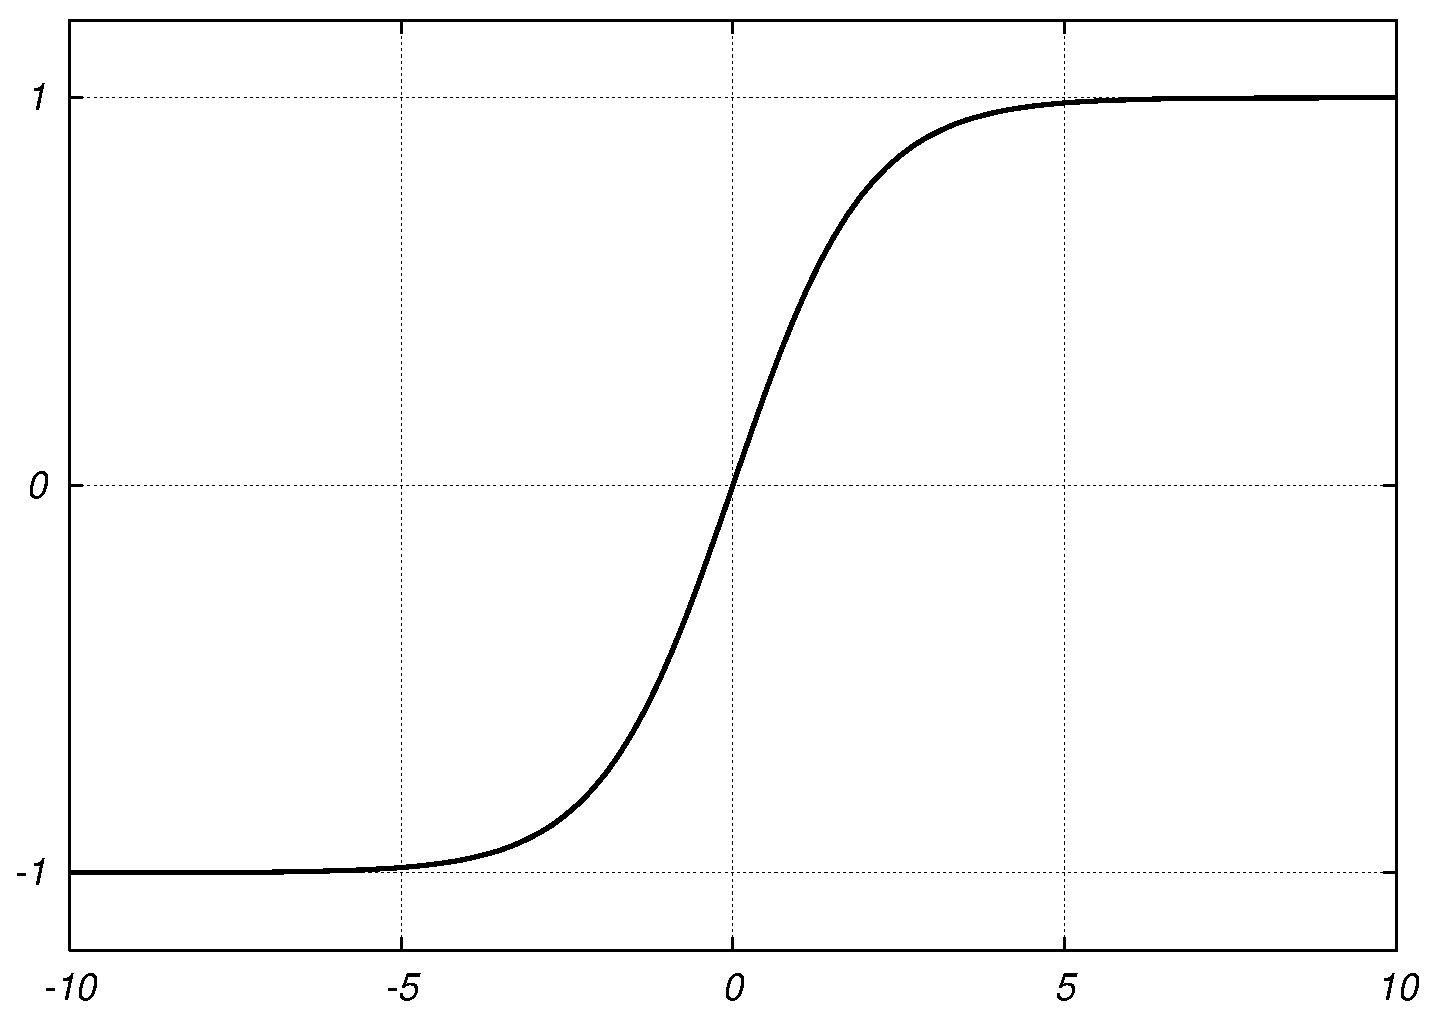
\includegraphics[width=0.45\textwidth,%
  totalheight=0.25\textheight]{tanh} &
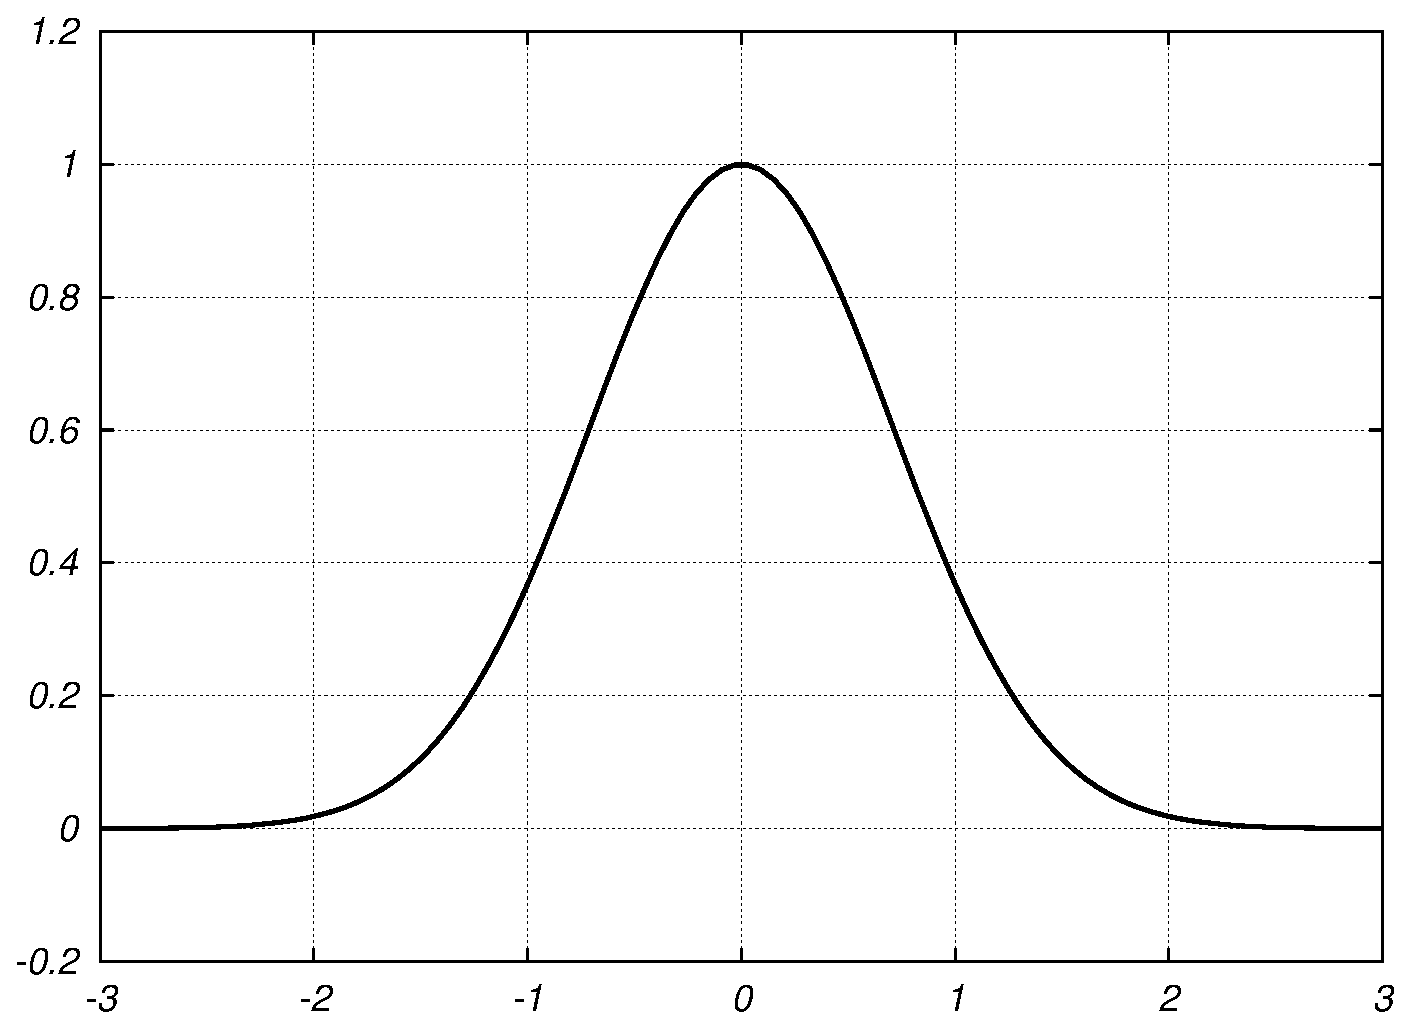
\includegraphics[width=0.45\textwidth,%
  totalheight=0.25\textheight]{rbf} \\
�) & �)\\
\end{tabular}
\caption{������� $\fa$ �������������� (�) � ���������-��������� (�) �����.}
\label{fig:act_func}
\end{figure}

���������� ������� ����������� ������������� ������������.  ������� �
����� ������ ���� ������������ � ���� ��������.  �� �����������
����������� ������� ���������� �������� � ���������������� �����
������, �� ����, ����� ������� ������� $i$-�� ���� �������� �� ������
�� �������� $(i+1)$-�� ����.  ����� ������������ ��������� ���� ���
������������ � �������� ������ ���������� �� \figref{fig:mlann}.

\begin{figure}[h]
\centering
% This does not make picture in PDF/LaTeX:
%\input{nn_arch.pic}
% So, let's do the next way:
% 1. xfig -specialtext -latexfonts -startlatexFont default nn_arch.fig
% 2. Update all text objects (with TeX special symbols) to Default font
% 3. Export to PS/LaTeX (changing default extension from .pstex to .eps)
% 4. Edit nn_arch.eps_t file and remove .eps extension from \includegraphics
% 5. Put next \input:
\input{nn_arch.eps_t}
\caption{������������ ��������� ���� ������� ���������������.}
\label{fig:mlann}
\end{figure}

��� ����������� �������� ����������� ������������ ��������� ����
������ ������������ ����������� $\NN_{n_0,n_1,\ldots,n_{m-1},n_m}$,
��� $n_0$ --- ����� ������ ������� (��������) ���� ����,
$n_1,\ldots,n_{m-1}$ --- ����� �������� � ���������������
������������� ������� �����, $n_m$ --- ����� �������� (� �������)
����������, ��������� ����.

%\subsection{����� ����� �������� � ����������� ����}

����������� ����� ���������� �������� � �� ������������� �� �����
�������� ������� ���������.  � ����������������, ���� ���� � �����
������������� ���������� --- ������� ������������� ��.  ��������
������������ ������ ������ �� ����� ��� ��������� ������� �������, ��
���� ���������� ���������� � ���������� ����� (��������, �������������
������ �� ������ �� � ���������-�������� ��������~\cite{koh80}).
����� ���������� �������� � ���� ������ ������������ �����������
�������������� �������.  � ����� ������, �� � ���������-��������
�������� ������� ���������� ������� �� ������ ���������� ��������, ��
� ��������� �������.  ��� ��������� �������� ���������������� ���
���������� � ������������ ����� �����, ����������� �������
������������ ��.

%\marginpar{����� �������?}
%�������� ������� � ���������������� ����������� ���� �������
%��������������� � ������������ $\NN_{n,k,m}$ � ������������� ��������
%���������~(\figref{fig:act_func}�).  ��� ���� ��������� ���������
%����������� ���������� �������� �������� ���� ��� ������� ������
%������������� $N$ ������� ��������� �������:
%\begin{equation}\label{eq:neuron-number}
%\displaystyle\frac{mN}{(n+m)(1+\log_2N)} \le k \le
%m(N/n+1)+\displaystyle\frac{m}{n+m}(N/n+2)
%\end{equation}

������������� ������ ������� ��������� ���� � ������������
$\NN_{1,n,1}$ ��� ����� ������������� � ������������ � ����� ����
������ � \cite{sontag93}.  ��� �� ����������, ��� ���������
������������� ��������� ����� ������� ������������� ��, �����������
�������� �����������, � ����� ������ �������� NP-������ ���������.

������, �������� ����������, ��� � ����������� ����������� ������� ���
������������� � ������ ��������� ������������ ����� ��������.
��������������� ������ ��� ������� ����������� ����������.  ������
������ ������������ ����� ���������� ����� ������������� �������� � �
������������ ������� ��������� �� ��������� ������ � ����������
�������.

��� ������������� �������� �� ����� ����� ��������� �������������
���������, ������������ �� ������������ ������.  � ���������,
��������, ��� ����- � �������������� ���� ������������� ����� �������
�������� ����������, ��� ����������� � ����������� ������ �������
�������������.  � ��� ������, ���� ��������� ���� �� ������ ����������
������, ������������� �������� �� ��� ����� ��������������� ����������
(���� ���������� ���������������, ��������� � ������������
��������~\cite{wasser92}).

�������� ����� �������, ������������� � ���������� ��� ��������
�������� ��� ���������� �� ������������ ���������� ��� �������
���������� ������~\cite{gibb96}.  ������ ������� ���������� ����
������� ��� ������� ����� ���������� ������ ����������.  ��������,
����������� � ���� ������� ��������� ������ � ������ ������������
��������� ���������������� ��������� ������.

%\subsection{������������ ����������� � ������������� ����������}

� ��������� ���� ������� ��������������� ����������� ������ ����������
������������ �� ������.  ��� �������� ������������ ������� ���������
����� ������������ ��������� �������:

\begin{itemize}

\item
������������ ������ �� ���� �� �������� � ���������������� �������
������� (\figref{fig:dynamic_nn}�);

\item
��������� �������� ����� � �������� ���� ��� �� ������������
������������ ����: ���� ������ � ��������~\cite{gibb96,golovko01};

\item
���������� �������� ����� � ��������� ����: ���� �������� � ��������
��������������� ������ �� �������
(\figref{fig:dynamic_nn}�)~\cite{wasser92,golovko01}.

\end{itemize}

\begin{figure}[h]
\centering
\begin{tabular}{cc}
\hbox{\input{dnn_arma.eps_t}} &
\hbox{\input{dnn_feedback.eps_t}} \\
�) & �)\\
\end{tabular}
\caption{������� �������� ������������ ������� ��������� ���� � �������
         ���������� �� ��������� ��� (�)
         � ���������� �������� ������ (�).}
\label{fig:dynamic_nn}
\end{figure}

% �������������� ����������� �� ������ ����

%\subsection{��������� �������� ��������� �����}\label{nn_learning_algorithms}

��������� ��������� ���� �� ������� ���������� ���������� ������
�������������� ����� ����������� ��� ����������� ��������� �������
$w_j$ --- ������� ������������� ��������.  � ������ ���������-��������
�������� ���������� ����� ������ $c_j$ --- ������ �������.  � ���
������, ���� ��������� �� ������� ��� ������� ������ �������������
��������� ����������� ������� $f(.)$, �������� ��������, �� �����
������� �������� ��������� � �������� ({\em supervised learning}):
\begin{equation}\label{eq:supervised_learning_task}
  \begin{array}{c}
    \mathbf{y}_k=f(\mathbf{x}_k)\\
    \sum\limits_k\big(\mathbf{y}_k-\NN(\mathbf{x}_k)\big)^2\rightarrow\min
  \end{array}
\end{equation}

������������ �������� �������� � �������� �������� ������
������������� ������� ``����������� ���''.  ���� �� ������� ������� ��
������ ����, �� ������� ��������� ��������� �������� �� ����������,
���� ������� ���������� ��������� ��� ������� ({\em unsupervised
  learning}).  �����, ��������, �������� ������� ������ ������������ �
������� ��������� ���� ��������~\cite{wasser92}.

��� ������� ����� ������� ����������� ������� �������, ������� ������
�������� �������, ��� �������, ������, ������� ����������
��������������� �������� ������ �������� � ��������.  ���� ���
�������� �� ����� ������ � �������� �����������, ������� ������� �
�������� ����� �������� �������� ������.  � ���������, ������
����������� ������ ����������� � �������������� (���������� ������).

������� ����������� ������� �������� �� �������� ��������
��������������� ������.  �� ������������� ������������ ������
����������� ������� �������, ��� ������� ��� ������ �����������
������������ ���������� � ������ ����������� ������� ������.
��������� ���������� ������, ��������� � ����������� ��������� ������
��������, ����������� � ��������� ������� ������� �������.  ����� ���
���� ��� ������������� ���������� ��� �������� �� (QuickProp,
Delta-Bar-Delta � �. �.), ��� � ������� ������ �������� � ������
����������� (������ ����������� ����������, ����������-��������� �
�. �.~\cite{himmelblau75}).  ������������� ����� ����������� �������
�������� �� � ��������� � ���� �������� ���������� �~\cite{gibb96}.

������ ������������ ����������� ������� �������� �������� �������
�������� ����������, �������� �������� ������� ������� �������.
������ ������������ ��������� ������ ����� �������� � ���������
������� ������ �����������.  � ����� ������ �������� ������
����������� �������� ����������� ������� �� ����� ���� ������.

�������� ������������ ������, � ������, ��������� � ��������� ��������
�������� � ������� ������ ������� ���������� ������.  ���� �� ���,
�������� {\it alopex}, ����������� �~\cite{boquete99}, ������� ��
���������� ������ � �������� ������� ������������� � ��������������
���������� ���������� ��� �� ���������� � ������ �����������.  �������
�������� ����� ����� ������, ��������� ��� �� �������� � ����������
���������-����������~\cite{wasser92}.  ������ ���������� ���� � ����
������ ������������ ``������������'' ����.  �� ���� ���������
����������� ��� ������������� �������������, ��� � ������� ����������
���� ������� ������������ ����������� ��������.  � ���������, �
������� ��������� ������ ���������� ������ ����������� ���������
�����������.  ����� ����, � �������� ���������� ������ ����� �� �����
���������� ������ ���������� �� �������� ��������.

������ ������� ������������� ���������� � ������ ������� ���������� �
����� ������ ������ ����������� ��������, ��� �������, ����������
��������.  � ������ �������, ����������� ������ ���������� � ���������
� ������������ �������� ����������� ������������ ���������� �
�������������� ������������ ���������� �������� � ���������������
������������� �����������.  ��� ����������� �������� ��������� ���
������ ����������� ������� �������� ��, ��� �������������� ��������� ��
������������� ������������� � �������� ��������������� ����������.

%%%%%%%%%%%%%%%%%%%%%%%%%%%%%%%%%%%%%%%%%%%%%
%\section{����������� ���������� ��������� ����� � �������� ����������}
\section{���� ��������� ����� � �������� ����������}

������ ���������� ����������, ��� �������� �� ������������ ��������
���������� ��������� ���� ����� ��������� � �������� ���������� �����
� ���������� ������ �����.  ������ ���� ����� ���� ���������, ���
����������� ������������ ���������� �� ����������� ��������� ���� �
�������� �� ��������.  � ����������� �� ������������� ����� ���������
���� ��������� � ����� �� ��������� �������:

\begin{enumerate}

\item
����������~\cite{sigom00,khomyu96,kav96,bouchard01,linwaihong01,gorfeld96,tukin01,pican95,golovko01,fabri98};

\item
������ ������� ����������~\cite{narmuk96,park96,levinar95,kulee96};

\item
������������ ������� ������� ����������~\cite{hayyeeder97};

\item
���������� ��������� � ����������� ������� ����:
��������~\cite{steck96,sigom00,chenmills97,vas-bak2009} �
�������-����������~\cite{sigom00,wailinlin00,linwaihong01};

\item
����������� ���������� ������� ����~\cite{sigom00,samtar96};

\item
�������������� ��� ��������������
�������~\cite{uhrig91,zhuchkov02,basubart94,golovko01}.

\end{enumerate}

� ���������� �� ����� ������������� ������ ������������� ����������� �
������������ �������, ��� ��� ��� �������� ��������������� � �������
�� ����� ���������� ����� ����������.  �������������� �������� ��
������������ ���������� ����������� � ����������� ��������� �����, �
����� ������������ ���������, � ����� ������� ���������� ������������
������ ������� ����������.

%\subsection{������������ ���������}
\section{������������ ���������}

%%%%%%%%%%%% �������� ��������� ����� ��������� �� ������

% ���������� �� ����������

������� ������������ �����������, ������������ ���������� �����
������������ ��� �� ����������, ��� � �� ����������.  � ���������,
������������ �������� ���������� �� ����������, � ������� ���������
���� ���������� ����� ������� ����������� ���� $\NN(e_k)$ (��������,
�~\cite{ronco98}).

% ���������� �� ����������

����������� ������������� ���������� $\NN(r_k)$, ��� $r_k$ ---
�������, ��������������� ���������� �� ����������, ����������� �������
������~\cite{khomyu96}.

% ����������� ���������� feedforward+feedback

��������������� ����� ��������� ������������� ���������� ������ �����
����������� ������ ���� $\NN(r_k,y_k)$, ��� $y_k$ --- ����� �������
����������~\cite{narpart92,trc95,samtar96}.  �������� �����������
��������� ����� � ���������� ������������� �������, ������������� ����
������� ������������ $\NN(e_k,y_k)$ � $\NN(e_k,r_k)$, ��� ���
$e_k=r_k-y_k$.  ������������ ��������� (��--�) � ������������ ������
$\NN(e_k,y_k)$ ������������ �~\cite{narmuk96}.

����� ���������������� ������������� ���������� ����������
�~\cite{sigom00}.  � ������~\cite{park96} �������� ����� ������������
��� ������������ ���������� ���������� ������������ ��������.  ���� ��
��������� ����� ($\NN^{FFC}$) �������� ����������� �� ����������, �
������ ($\NN^{FBC}$) ���������� ���������� �� �������� ����� �������
���������� � ���� ����� �������� �����.  ����������� ����������� ��
������ ����������� � ������������ � ����������:

$$
u_{k}=\NN^{FFC}(r_k)+\NN^{FBC}(r_k, y_k, u_{k-1})
$$

\noindent
��� $r_k$ --- �������, $y_k$ --- ����������� ����� ������� ����������,
$u_{k-1}$ --- ����������� �����������, �������������� � ����������
������ �������.

% ������ �����
� ��������� ������� ������������ ��--� � ������������ ���������
�������� �� ������� �������� �� �����.  ��������, �������� ����������
���� ���� --- ���������� ������������ ������� � ��������� ���� �������
���������������.  ��������, ����� ������� �� ���� �������������
���������� �������� ���������� ����������� ������� � ������� ��������:
$\NN(r_k,\dot{r}_k,\ddot{r}_k)$.  ���� ������� ������������� �
�������� ������ ����������� ������� ������:
$\NN(e_k,\dot{e}_k)$~\cite{wailinlin00,linwaihong01},
$\NN(e_k,\dot{e}_k,\ddot{e}_k,\ldots,{e}^{(n)}_k)$~\cite{eremin95}.  �
��������� ������ ���������� ����������� $n$ ������������ ��������,
������ �� ������� �������.

�������� �� ������ ���������� � ���������� ������������� ��������
��������� ������������� ���������� � ������ ����������, ��������
�������� ������ � ��������� ������ ��� ��� ���� ����� � �������������
���������� ������ ��� ������� ������.  �� � ����� �� �������������
����� ������ �� ������������� ����� ������, �������� �� ��������
���������� ��������� �����.  ��� �������, ����� ����� � ������������
������ ��--� �������������� �� �������� � ���������� ������������ ���
�� ���������� �����������.

% ��������
���������� ������������ � ���������� �������� ������� ���������
������������� ����������.  �� ���������� ������ ������� �����
���������� �~\cite{sigom00}.  �������, ��� � ����� ������ ������
�������� �� ������� �� ���� � ���������� ������ ��--�.

%\subsubsection{������ ��������� �������������}%
\label{direct_inv_nnc}

������ ��������� ��--� � �������� ���������� �� ���������� ��������
��~\figref{fig:direct_nnc}�.  ���� ����� ������������� ��� �������
���������� �� ����������� ������.  ��� ���������� ������������ �������
������������ �������� ����������� �� ���� ��--� ����������� �� �������
����������� �� ������ ������� ��������~\figref{fig:direct_nnc}�.  �
�������� ��������� ��������� ���� ��������� ������ �������� �������
����������.  �� ��������� �������� ��--� ���������� � ������
����������, �� �� �� ���� �������� �� ����������� ��������
$y_k,y_{k-1}$, � �������� $r_k,r_{k-1}$.  ����������� ��������,
��������� ���� ���������� ����� ����������� ����������� $u_k$, �����
����� ������ ���� ������ ���������.

\begin{figure}[h]
\centering
\begin{tabular}{c}
\hbox{\input{nnc_direct_inv_tr.eps_t}} \\
�) \\
\hbox{\input{nnc_direct_inv_ev.eps_t}} \\
�)\\
\end{tabular}
\caption{������ ��������� �������������: ����� �������� (�)
         � �������� ���������������� (�).}
\label{fig:direct_nnc}
\end{figure}

�������� ����������� ����������� ����� �������� ������������� � ���,
����� ������ ���������� ��� ���������.  ��� �� ������ ����� �����.
����� ����, ������ ���������� �������� ������� ������� ����������
�������� �������� ������� ���������� � ������� ��������
������������������ �������, ������������� ��� �������� ��--�.  �����
����� ��������� ������������� ������ � ����������� ����������� ������
� �������, ��� ������ �������� ��������� ���� ����� ����������
����������.  �������� ��������� �������� �������� � ������� ��������
��������.

%\subsubsection{������������������ ��������}

������ ����� �������� ��--�, ����������� ��~\figref{fig:special_nnc}
(��� ���������� ������������������ ��������), ������������ ����������
������� ������������� ��������� ���� � �������� �� ��������
����������������.  ����������� �������� �������� ��--� ����������
���������� �� ������ ���������� � ������������ ������ ���� �������.
��� ���������� ������ � ������ ������������� ���������� ����������
����� ���������� �������� �������� ������� ����������.  ��� �� ������
��������, ������� ����� �������������� ������ ��������, ������������
�����������, � ������� ���� �������� ����������� ����������� ���
���������� ������ ����������.

\begin{figure}[h]
\centering
\input{nnc_special_tr.eps_t}
\caption{����� ������������������� ��������.}
\label{fig:special_nnc}
\end{figure}

��������� ����������� ���������� ������� �������� ����������������
������ ��������� ���� � ������ ������ ��������.  ���������
������������ � ��������� ��--� ��������� ��������, �� ���� ���������
�������� $u_0$ ����� �������� � �������� ������� ���������� �
���������������� ������������.  �������� �� ��, ��� ������ �����������
� ���������� �� ��������������, ��������, ��� ������������������
�������� � ������ ���� �� ��������� �� ��������.

%\subsubsection{��������� ���������� �������������}

��� ��� ����������, ������ ����������� �������� �������� �������
���������� ������������ ������������ ���������.  ���� ���� ����������,
� ����� ������ ������ �������� � ������� ��������� ���� ���������� �
�.~\ref{identif_and_nnp}.  ������� �������� ��--� � ��������������
������������ ������ ��������~(\figref{fig:indirect_nnc}) � ������
������� ���������� ��-�������: ��������� ����������
�����������~\cite{narpart92}, �������� ���������������� �� �������
(������), ��������� � ���������������~\cite{sigom00}.  ���������������
�������� ����������� �� ����, ��� ������ ������������ ������ ������
���� ������������ ���������� � ���� �������, ����� ���� ��������������
����� ���� �� ����� �������� � ������������ ������ ����������.

\begin{figure}[h]
\centering
\input{nnc_indirect_inv_tr.eps_t}
\caption{����� ���������� ����������� ������������� �������������.}
\label{fig:indirect_nnc}
\end{figure}

� ������� ������ ����� ���������� ������������������� �������� ��
����������� ������� ������ ��������.  ������ ������ �������������
������������� ��������� ������ ��������� ���������� ����������
����������� ������ � ���������� ��������.  ������������ ������ �������
���������� (��--�) ��������� �� ����� ��������� ��������������� ������
������� ������� ���������� �����, ��� ��������� ��� ����������
������������ ���������� � ���������� ������������ ��������� �������
��--� � ��--� ������������.  ��������, ��� ���������� ����� ���������
����� ��������� ������������ ������� ���������� � ��������� ����������
������� � ������� �������.

�������, ��� ���������� �������� ������� ���������� �������� ���������
������� �������� �������, ������������ �� �������, �������������� �
�.~\ref{direct_inv_nnc}.  � ������� �� ������ �������� ���������
����������� ���������� ��������� ��������������� ������.

%  � ������� �� ������ �������� �����������
%������� ���������� �� �������� ������������, ��� ��� �� �����
%��������� ��������������� ������ ���������� ����� ��--� ������������
%���������� ������ ��������, ��������� � �����, ����������� �������
%��������� �������.

����� ��������������� ����� ������������� � ����� �� ������� ��������
��������� ����� � ��������� ������� --- �������� ���������������� ��
������� ({\it backpropagation through time --- BPTT}).  ������, ���
������������� ���������� �� ��� �������� ������ �������� ����������
���������� ����������� ���������� ������ � �������, ����� ��������,
��� BPTT, �������� �������� ��������� �����~\cite{narpart92}.

� ������~\cite{fabri98} ������������ ������������ ����� ������������
�������� ������������� ����������, ���������� �� ������������
���������� �������� ����������.  ��� ���� ���������������, ���
������������ ������ ������� � �������� ��������� �������������
������������� �����.  ����� ������������ ��� �������������
������������� ����������� �������, �������� �� ����������, � ����������
������� � ������ ����������.  ������������� ����������� ������ ��
��������� � ������� ������� �������� ���� ���������������� ���������
������� � ������ ������� ������� ������ ���.  ��������������� �������,
���������� ��� �� ������������ �����������, ��� � �� ���� �������� �
���������-�������� ��������.

%\subsection{������������ ������ ������� ����������}

%� ���������� ������ ��� ������� ������ ������� ������������� �������
%���������� ���������� �������� ����� ��� ������ �������� ��������
%����� ���� ����� �������.  ���� ``����--�����'', ����������� �� �����
%���������� �� �������� �������� ��������������� ���������� �����
%������������ � ���������� ��� ��������� ��������� ���� ��� �������
%������� ����������-���������.

%\subsection{������������� � ������������ ������ ������� ����������}%
\section{������������� � ������������ ������ ������� ����������}%
\label{identif_and_nnp}

��� ������� ������������� ����������, ������������ ��������� �����
����� ����������, ��������� ������ � ������������� ��������� ������
���������� �� ��������� �����.  �� ������ ���������� ��������, ���
������������ ��������� ����������� ����������� �� ������ ����� ����
���������� �������� �������� --- ������� ������� ����������� �������
��������� ������� ���������� �� ���������� ������������ �����������.
����� ���� �������� �������� ������� ������� ���������� �� ��������
��������� � ��������.

� ������������ �������� ������� ����� �������������� ������������ ��
������ ������� � ��� �������� ����� �������������� ��� ���������
��������� ���� ����������.  ������ ��� ����������� �������� ��������
���������� ������ ���������� �������� ��� �������� � ������� �������
�������������.

������������ ����� ������������� �������� ������ ����������
������������ �� ������������ ����������� ��������� ������� ��
���������� �������������� � �� ��������� �������, ����������� ���
��������� ���������� �������.  ������ ������ � ������ ���������
�������������, ��������� ���������� �� ���������� ������� ��������.

����� �� �������� ����������� � ������� ��� ���������� �� �����������
����������� ������� ������������� ����������� ���������� �����������
������ �������� �������� �������~\cite{bolonchin91}.  �� ���������
���������� ���������� ������� $A$ ����������� ���������� ��������
���������� ������� ����:
\begin{equation}\label{kachmaj}
\mathbf{x}_k=A^T \mathbf{u}_k
\end{equation} ��� $\mathbf{u}_k$ --- ����������� �����������, �
$\mathbf{x}_k$ --- ����������� ��������� ������� ����������.

������ ����� ������������� ������� �~\cite{boxjenk74}.  �� ������� ��
���� ������, �� ������ �� ������� ����������� ������� � ���� ������
�������, � �� ������ ���������� ��������� ������ � ����������� ��
�������������� �������������.  ������ �������� � ����� ���������
����������� ���������:
\begin{equation}\label{arima}
x_k=\delta^{-1}(B)\omega(B) u_{k-b} + n_k
\end{equation} ��� $B=1-\nabla$ --- �������� ������ �����, $n_k$ ---
��������� ������, ����������� ��������� ����, $\delta$ � $\omega$ ---
��������.

������������� ������ ����������� ������� � ��������� � ����������
������������ ������� ���������� � �� ���� ������� ����� �������� ���
������������� ���������� ��������, �������� � ��� ������, ���� ���
������������ �������� ����������.  � �� �� �����, ������������
��������� ��������� ����������� ���������� �������, ������� ���
���������� ������ ������������� ��� ��� ����� ����� �������� ������
�������� ����������.  �� ���� ������� ������������ ���� ������
���������� ������ ������� ��� ���������� ����������� �� �������������
��� ������ �������� ����������� ������������ ������� ����������
������������� �������������, ������ ��� �������� ��� ������ �������
������� ����� ����������.

%%%%%%%%%

���������� ������������ �������������, ��� ������������ ������������
������� � ��� �������� ���������� ����� ������ �������� ��� �������
������������ �����������.  ��� �������� ���������� ������ ����������,
����������� ������� SISO ({\it single input, single output} --- ����
���� � ���� �����).  � ���������� ������� � �������� ������������
��������� ������ ���������� ����� ����������� ��������� ��������
���������� ���������:
\begin{equation}\label{eq:siso}
\left\{\begin{array}{rcl}
  \mathbf{x}_{k+1} & = & f(\mathbf{x}_k, u_k) \\
  y_k & = & g(\mathbf{x}_k)
\end{array}\right.
\end{equation} ��� $y_k$ � $u_k$ --- �������, � $\mathbf{x}_k$ --- ������
��������� ������� � ���������� ������ ������� $k$.

��������� ���� ������� ���������������, ����������� �������
$\hat{y}_{k+1} = \NN^o(u_k)$, ������������� �� ����� ������ ������
�������� ��������� ������������� ������� \eqref{eq:siso}, ��� ���
��������� �� �������� �������: � ����� ������ ����� ��������� ����
������� ��������������� ��������� ������������ � �����������
������� � �� ������� �� ��������� ��������� � ���������� �������
�������, � ����� �� ������� ������.

��� ���������� ���������� ������������ ������ ������� ��������
��������� ����������� � ������� ����������.  � ���������� ��
������������� ���������� �������� ��������� �������� ������� ����
��������.  �������� ��������� �� ��� ������������ �������������
�������� ������ ������ ��������� ���� ��� ���������� ��������� �����
�������� �������.  ������ ������� � ���������� ������� �������� ������
� ������� ��������� ������� ���������������.  ������ �������
������������ ���������������� ���������� ���������� ������� ����������
� ����� ``���������'' ��������� � ��������� ������������� ������� �
���������� ������� �������.  ��������� ��������� �������� ������,
������������ ��� ����������.  ���������� �� ���������.

%\subsubsection{���������� �������� �����}

���� �� ��������� ��������� ������ � ���������� ���������� ���������
���� ��������� �~\cite{boquete99}.  ����������� ��������� ������������
������ ������������ ����� ����������� ������� ���������-�������� ����
� FIR �������� � ��������� �������� �����.  ���������������� ������� �
������������ ������ �����������
����������~\eqref{eq:rbf_neuron_output}, ������ ���������-��������
������� $R(.)$ ����������� �� ����� ������� �������, ����������
��������� �������� �����:

$$
R_j\bigl(\mathbf{x}(k)\bigr)=
   \exp\Bigl[-\frac{1}{\sigma^2}\sum\limits_{i=1}^M
             (x_i(k)+\tilde{x}_{ji}(k)-c_{ji})^2\Bigr]
$$

$$
\tilde{x}_{ji}(k)=\sum\limits_{s=1}^S a_{jis}R_j\bigl(\mathbf{x}(k-s)\bigr)
$$

��������� ����� ��������� ���� ���������� � ������� ���������������
������������ ������ � ����� ����� ��������� ������� �������������
��������� ���� $w_i$ � FIR ������� $a_{jis}$.  �
������~\cite{boquete99} �� ���������� ������������������ �������
������ ������� �������� ����� $S$.

������ ������� ������������ ������, ������������ �~\cite{benne00}
����� ����������� ���� ������~\cite{golovko01}.  ��������� ���� �����
������� �����������
$\hat{y}_{k+1}=\NN^o(u_{k-1-n_L},\ldots,u_{k-n_b-n_L})$, ��� $n_b$ ---
�������� �������� �������� ���������, $n_L$ --- �������� ��������
�������� ������������.  ����������� ���� ������� �� $n_a$ ��������
$\hat{y}_{k},\ldots,\hat{y}_{k-n_a+1}$.  ��������� �����������
������������ ������ $n_a$, $n_b$, $n_L$ ������������ ��������� ��
��������� ��������� ������ �� �������.

%\subsubsection{������� �������� �����}

������������ ������ ������� � ������ ������� ������� ����������
�������������� ������, �� ������� �������� ����� ������,
���������� � ���������� ������ �������~\cite{sigom00}:
$$ \hat{y}_{k+1}=\NN^o(u_k, \hat{y}_k) $$

����������� ������ �������� ����� $\hat{y}_k$ ����� ����� ������
���������.  ����� ������ ���������� ��~\figref{fig:nnp-feedback}.

\begin{figure}[h]
  \centering
  \input{nnp_feedback.eps_t}
  \caption{������ � ������� �������� ������.}
  \label{fig:nnp-feedback}
\end{figure}

��� �������� ��������� ����� � �������� ��������� ������� �����
������������ ����� ��������� ��������������� �
�������~\cite{gibb96,sigom00}.

������������� � ��������������� ������ ������ ������ ����� ��
������������, ��� ��� �������� ��--� ��������� ������ �������
��������� ��� $(u_k, y_k)$, ���������� ��� ���������� �������� �
��������� �������.  ��� ������ ��� �������� � ��� ����������������
������ �� ������������.  ��� ��������, ��� ����� � ������ ���������
(��������) ������ ����� �� ����������.  ������������ ������ ������� �
������ ������ �������� ��������� ����������.  ��� ��������� {\it
��������� }�������.  ������� �������� ������������� ���������� ��
������������ ������ ��������� �������� ��� ������� ����������.

������ � ���������� ���������� � ���������� BPTT.  �������� ��������
�������� ����� ������� � �������������� ��������� ����������, �������
����� ������ ��� ���������� ������� ��������� ���� �� ����������
����������� ������� ��� ����������� ��������� � ��������
�����������~\cite{levinar95}.  ����� ����, ����������, ��� ��������� �
�������� ��������� ������� �������� �������� ����������� � ���������
������������������, �� �� ����� ��������� ������� � ���� �������������
���������� ���������� � ����������� � �������� ����� � ��������
��������� ��������������� ������~\cite{linetal}.  ��� �������� �������
�������� ����������� ��������� ({\em vanishing gradient}).

������������� � ������ ������������ �������� ������� ����������
�������� ����������� ��������� ��������� � ���� �������:
\begin{itemize}\label{simple-feedback-defects}
  \item ������������ ������ ������������ � �������� �������
  ����������;
  \item ��� ����������� ������� ������� ��� �� ��������� �
  ����������� �������� ����������� ��������������� ������.
\end{itemize}

%\subsubsection{���������� ������� ���������}

�������� ����� ������ ��--� ����� ��������, ���� ������������ ���
������������� ������������� �������� ������� ��������� ������� ���
���������, ������� ��������������� ����������� � ���������� �������
�������.  � ���� ������ ������� ������ ������� ���������� ������ ���
�������� ������ �� ������ �������� ���������� �� ������� ����������:
\begin{equation}\label{eq:past-states}
  \hat{y}_{k+1}=\NN^o(u_k, u_{k-1},\ldots,u_{k-D_u}, y_k,
                           y_{k-1},\ldots, y_{k-D_y})
\end{equation}

������ ������ ����������� �� ������ �������, ��������
�~\cite{kulee96,levinar95}.  ����� ����� �� ��������� ������� �
����������� ������� ��������� ����������
��~\figref{fig:nnp-past-states}.

\begin{figure}[h]
  \centering
  \input{nnp_paststates.eps_t}
  \caption{������ ������ � ����������� ������� ���������
  $\hat{y}_{k+1}=\NN^o(u_k, y_k, y_{k-1})$.}
  \label{fig:nnp-past-states}
\end{figure}

�������� ���� ������ �������������� ��� ������� ���������� ��
��������� �������� �������, ���������� ��������� ���� $u_k$ � $y_k$.
��������� ���� $\NN^o$ ��������� ������ ������� ���������
������� ����������� ������ � ������� �������������� ��������.
��������� � ������ ����� �������� ����� �����������, ��������
������������� ������ �� ������� �������� ����������� ��������� �����,
��������, ������������ ������ ��������� ���������������.

����� ������ �������� ����������� ��������� ����� �������������� �
������� ���������� ��� ������������ ������ ������� � ��� ���������
���������������.  ����� ������ �� �������� ����������.  ��� ���������
�� ���������� �� ��������, � �� ��������������� �� ���������� �����
��������� �������.  ����� �������, ��� ������ {\it ������������
}������ ������� ����������.

������ ���������� ������� ��������� ����� �������������� ��� ��������
������� ����������, ������ ���������� �������������� ������ ����������
������������ ����������� ��������� ������� ���������� ��� ���
�������������� �, ������, ��� �������� ���������������.  �����
�������, �������� ������������� ���������� ������ �������������� �
������� ���������� � ������ �������� ����������������.

%\subsubsection{��������� ������}

������� ��������, ��� �������� ����������� ����� ������� � ������
������� ���������� �������, ����� �������� ������������
��~\figref{fig:nnp-hybrid}~\cite{park96}.  �� ����, � ������
����������� �������:
\begin{equation}\label{eq:nnp-hybrid}
  \hat{y}_{k+1}=\NN^o(u_k, u_{k-1},\ldots,u_{k-D_u}, \hat{y}_k,
                              \hat{y}_{k-1},\ldots, \hat{y}_{k-D_y})
\end{equation}

\begin{figure}[h]
  \centering
  \input{nnp_hybrid.eps_t}
  \caption{������ ��������� ������
  $\hat{y}_{k+1}=\NN^o(u_k, \hat{y}_k, \hat{y}_{k-1})$.}
  \label{fig:nnp-hybrid}
\end{figure}

��� �������� ��������� ���������� ������������ ����������� ��������
��������� ��������������� �� �������, ����������� ��������.

� ������ ������ ��������� ������� ����������� ������ � ��������
��������� �������.  � ���������, ����������� �� �������� �������
������������ ����� ������������� ����������� ������ ������ ����������
������ ����������, � �������� ����� � ����������� ����������
����������� ������� ��--� --- ������.

�� ��������� � ������� ���������� ������� ��������� ������� ����������,
��������� ������, ��-������, �������� ����������, ��-������, ���������
���������� ����� ������ � ����� �������� �������� �������.

������ ���������� ��������� ����� ��� ���� ������������ ������������
���������� ������� � �������� ��������� ������� (� ��� ����� �
���������).  ��� ��������� �������� �������� ���������, �� �������
���������� �������� �������� ��������� ��� �������� ������.

%\subsubsection{������������� ������}

� �������~\cite{narmuk96,ronco98} ������������ ������������
��������� ������� ������������, ������� � ������ ������ ������� �� ��
���, ������� ���� ��������� ����������� ������������ ������ �������
����������.  � ������~\cite{ronco98} ��� ������ ������ ������������
���������-�������� ��������� ����.  ��� ��������� ����� ������������
��������, ����� ������ ����������� � ����� ����������.

����������� ������������� ������� �� ������������ ��������� �����-����
������� �� �� �����������.  � ���������, ��� ����� ���� ���
������������, ��� � ������������ ������.

%\subsubsection{���������� ���������� ��������}

������������ ������������ ������� ��������� $E=\frac{1}{2}(\hat{y}_k -
y_k)^2$, ������������ ��� ��������� ������������ ������ ������� ���
������� ����������, ������� ���������� ������� �����������������
������� ��� ��������� ���������� ������.  ��� ����������� ����������
������ ������ �������������� � ������������ ��������� ������� �������
�������.  � ������~\cite{wangbao00} ��� ����������� ���������� SISO
������ ������� ������������ ������������ ���������������� �������
���������, ���������� ��������������� ������ ������ ��������:

$$
E=\frac{1}{2}\Bigl\{\bigl(\hat{y}_k - y_k\bigr)^2 +
  \lambda\bigl(\frac{\partial\hat{y}_k}{\partial u_{k-1}} -
  J^B_k\bigr)^2\Bigr\}
$$

\noindent ��� $J^B_k$ --- �������������� ������� �������, �������������
������������ $-J^B\le J^B_k\le J^B$, � $\lambda$ --- �������
�����������, �������, ��� ������������ � ������, ������ ���� ������
�������.  ���������� ��������� ������ ������������� �������� ��������
��--� � ��--�, ������������� ������������ �������� �������������
��������� ��������� �����.  ������������� ������� ��������������
����������� ������������ �������������, ���������� �� ����������
�������� � ����������� �������.

%%%%%%%%%

\section{������ ������� ���������� ��������� �����}

%\subsection{���������� ������������� ����������� ��������� �����}

��������� ���� ����� ������������ � �������� ���������� �����������
��� ��������������� � ������������ ������ �����, ������ ��������� ���
�����������~\cite{steck96,sigom00,chenmills97,vas-bak2009}.

����� ������ ���������� ������������ ������������ ����������� �
������������� ��������:

\begin{itemize}

\item
������������� ����������� � ������� ��--� ���������� ��������,
������������ ��� ������������ �������������;

\item
��������� ������� ���������� � ���������� ��������� ������� �������
��� ����� ����� ���������� ��--�;

\item
������������ ������� � ��--� ����������� �������� ������� � ���
�����������;

\item
���������� � ������� ��������� ���������� ������� ������������
��������� ������, ����� ����������� ��� ����� ������������
�������������.

\end{itemize}

��������, ��� ���������� �������� � ������������ ����������� ��������
�������� ���������� ����������� ����� ��������.  �������� ������� �
���� ������� �������� ��������� ������� ������������ ����������� ��
��������� � �������������.  � ��������� ������� (��������,
\cite{chenmills97}) ���������� ��������� ����������� ��������
������������ �����������.  � ������~\cite{warwick96} ��������� ����
����������� � ������� �������������� ������������ �������� ������
����������, ��� �������������� ������� �� ����� ���������� �������.
% ������������� �������� ��� ������������������ ���������
������~\cite{khomyu96} �������� ���������� ��������� �����������
���������� �����, ������ �������������� ���������� ����� ������������
��������, �� ����������� ������� ������������ ������� �� ����������� �
����� ���������� �������.  ������ � ���, �� � ����� �� ���������
������ ����� �� ���������� ���������������� ��������������
������������, ������������ ����������� �������� ������������ ��������
� ������������ ����������� � �������.  ������������ ������
������������ �� �������� ��������, ��� ��� �������� ������� ���
��������� �������, ��� � �������������� ��������� �������������� �
���������.

� ���������� ����� ����������� ������� ���������� �������
�������-���������� ����������� � ���������
�����~\cite{sigom00,linwaihong01}.  ����������� ������ ��������������
�� ������ ���������-�������� �����.  ������� ��������� � ���� �����
����� �����, ����� ������������ ��� ����������� ��������
��������������.  ����� ��������� ������� ���������-�������� �������
�������� ����� ����� ������������� � ����� ������ �������-�����������
�������.  ������ �������� ����� ����������� ����������� ������������,
� ��������� ������������ ��������� ���������� �����������
����������~\cite{wailinlin00}.  � ���� ������ �������-����������
������������ ��������� ������� ����������� � ��� �����������, ���
��������� ������������� ������������ ������� ������������ �
����������� ����������� ������, ���������� � ��������������� �������
����������.

%\subsection{����������� ������������ ����������}

������� ����� ��������� ������ ���������� ��������.  � ����������
������ ���������� ��������� ������������� ������� � ����� �� ��������
��������� ����������� ������ �������� � ������� �����������
����������.  � �������������� �������� � ������ ���������� �������
������ ���������� ������� �������� � ������� ������� �������.  ��� ��
�����, ���� ��������, � ������� ���������� ������������ ����������
������������.

������������ ������ � ����������� ���������� ���������� ����������
�~\cite{hayyeeder97}.  ������ ����������� �������� ������ � ������
������� � ���������� ������ �� ������ ��������� ���� �
���������-��������� ���������.  � ������ ���������� ����������
��������� ���������� ������������� ������� � ����������� ����������
�������.  ������������ ����� ������ ������������� ������������� �
������ ������������ ��������, ������������ ����� � ���������� ��
������������ ����������� � ��������� �������.


%\subsection{��������� ���� � �������� ����������� ����������}

� ��������� ������� ������������ ������������ ���������� ��������
��������� ����� �� ��������, � �������������, ��� ��������� ����������
������� ����.  ��������, �~\cite{samtar96} ��������������� ���
�������� ������� ���������� ��� ���������� � �������������� ���������
����.  ������ ������ ������������ ����� ����� ���������� �����������
���������� � ���������� ������������ ������� �������, ������������ ���
��������� ��� ����������.  ���� ������� ������� ����������� � ���,
����� �������� ������������ ������ �� ��� ��������� ���������
���������� �������������� ����������: $K_P$, $K_I$, $K_D$
(��.~\figref{fig:nn-tunes-pid}).

\begin{figure}[h]
  \centering
  \input{nn_tunes_pid.eps_t}
  \caption{��������� ��� ���������� � ������� ��������� ����.}
  \label{fig:nn-tunes-pid}
\end{figure}

� \cite{sigom00} ���������� ������� ����� ��������� ��� ����������,
������ � �������� ������ �� ������������ ������������ ������ $r_k$,
$u_{k-1}$, $y_k$.  ��������� ����������� ��������� ������������
������������ ������� ��������� $E=\frac{1}{2}(r_k-y_k)^2$.

������������ ������ ������������ ������������ ������������ ������� �
������ ������ ��������� ������� ����������.  ������������� ���
���������� �������� ������ ������������, ������ ��� ����������
�������� �� ������ ������� ������������ ��������� ����� �����
�����������.

\section{������������� ������������ � �������� �����������}

����������� ������������ ������� ���������� � ����������� �����
�������� �� �������� �������� ������ ���������������
�������������~\cite{warwick96}.  ��� �������� ��� ������� ��������,
��������������� � �������� �����������, ��� � �����������, �
����������� �����, ��� (�� ���� � ������, ��������, ����������
84\%~\cite{sigom00}).  ������� ��������, ��� ��� ��������� ��������
�������� �������� ��� ������������� � ����� ������������ �� ��� �����.

�������� ������~\cite{vukobrat1991} �� ������� ���������� �����
������������� ������ ���������� �������������� ������������� ������
��������� ��� ����������� � ������� ��������� ���� ������������ �
������ �����.  �������� �������������� ������������ ������� ��� ������
������� ������ ���������� ��������� ������ �������������� �������, �
��� �����, � �������������� ��������� �����.  � �� �� �����, ���������
���� �������� ����������� ���������� �������� � ��������� �� � ������
���������� ����������� ������ �������� ���� �������.

� ������~\cite{khomyu96} ���������� ���������� �������������
�������-�����������, {���������\-��\-��}, �� � ��������� �����������
���������� ({\em general predictive cont\-rol\-ler}).  ���������
�������������� �� ������� ���������� ������������ � ��������.  ������
������������ ��� �������� ������� ���������� (����������� � ������
������� ����������, ����������� �������������, ��������������
��������� ������������ ����������), ��� � ��������� ���������� �
��������� ��������� (����������� �������, ������� ������, ���������
������� �������� ������� ���������� � ������ ��� ����������).
�������� ����������� �������� ���������� � ��������� ����������
����������� �����������.  ������, ���������� � �������������� �������,
����� ��������������� �������� (``�����'', ``������'', ``������'',
``����� ����''), ��� ��������� �������� ������� ����� ������
������������� ��� �������������� ������ ���.  ������ �����������
���������� � ���������� ��������� ��������� ����� � ���������
��������� � ������� ������������.  ������ ���������� �� ����
���������� ������� ������ ���������������� ��������������� �����������
�� ��������� ���������, � �� ����� ��� ���� �������� ��������� �������
��������� �� ����������� �������� �������� ������ ��� �������������� �
������� ��� ������ �����.  � ������ ������ ��� ��
�������~\cite{sigom00} ����� �� ���������� ����� ��������� �������� �
����������� �������������, �������������� ���� ���� ��������� ��������
���������� �� ��������� � �������� �������.

� ������~\cite{boquete99} ���������� ������� ������ �������� � �������
�������� � ������� ��� ������������� � ������������ ���--��
�������������.  ����������, ��� ���������� �� ��������� ���������
����������������� � ��������� ������ �������, ��� ��������������
������� ��������� ����.  ������ ������ �������� ������ ��������
���������� � ������ �� ����������.

������ ������ ������������� ��������� � ������������� ����������
����������� �� ������ ���������� ������������ ����������
�~\cite{wailinlin00}.  ������ ��������, ��� ������ ����������
���������� �������������, ������ � �������� ������������ ����� �����
����������, ����������� ��������� �����������, ����������� ����������
�������� ���������� � �� ����������� � �������.  ���� ����� ����������
������������ �~\cite{vukobrat1991}.  ���������� ���������
������������--��\-���\-��\-��\-��\-��\-���� ���������, ������������
�������� �~\cite{wailinlin00}, ��������� ���������� � �������� �������
���������� � ������������ ������, �������� ��������� �����������������
��� ����������� �������� � 3 ���� �� ��������� � �� ���������.
������ �� ���������� ���������� � ����� ����������� ����������
����������� �������� �� ��������� �������, � ������������ ��������� �
������ ������������� �� �������� ����������� ��������������������
������.

����� � ������� �� ������������� ������������� ��������� �
������������� ������������ ����� ���������������� ��������, ��� ����
�������������� ���� ��������� �������� ������������� �� �����������
��������.  ����������� ������������, ��������������� ������������
�������� ����������� ����� ������������� � ��������� ��������
�����������.  ��������, ����� ������� ������ ����, ������ ��
���������� � ���������� ��������������� � ��������� ������ �� ����������
�� � �������� ����������.

������� ����������������� � ������������� ���������� ����� ���������
����� � �������� �������� ��������������� � �������~\cite{warwick96} �
\cite{toudeft}.  � ������ ����������� ����������, ��� ����������
�������� ���������� ��� ������������� ���������� �������� ����������
����������� ���������.  ����� ����� �������� ������������ ����������,
������� ���������� ������� ��������� �������� �, ��������� ����������
���������� � ��������� ��������� ����, �������� � ������ �
������������� �������������� �������� ������ � ������� ���������
�����.  ��� ���������, ���������� ����� ���������� �������� �
���������� ���������� � �������� �������� � ���������� ������ �������
�������� ����������.  ���������� ������ �� ����� ��� ��������, �����
����� �� ����� � ������ ������������ ���������� ��, ��� ������� ����
�������������� ������� ��������� ������������� ��� �������� ��������
�������� � ���������� ���
(��������,~\cite{khomyu96,wailinlin00,elfil-pta99}).

�� ������ ������~\cite{toudeft} ��������� ��--� �������������� ��
����� ���������� ����������� ���������� �������� ������������ ��������
� ������ �������������.  ��� ������� ��--� ������� ������� ���������
���������, � ������ ������������ ������������ ������������ ��������
������� �� ����������� ����������.  ����������� ������ ������ � ���,
��� ��������� ���� ��--� � ��--� ������������ �� ������ ������� �
�������� �������.  �������� ����� ���������� �������� �� ����
��������, ������� �������������, ��� ������ �������� ���������� ������
������ ������������� ������������� ������� ``������������'' ������� �
������ �������� ����������.

��� ������������ �������, ��������, �������� ���������������������,
��� ��� � ����� ������� ���������� ��������� ���� ������������ ��
��������.  ��� ���������� ���������� --- �������������� �
������������� --- �� ���� ������������� � ���, ��� �� ����������
��������� ���� � ������ ���������� �������� ��������.

�������������� ���������, ��� ��������������� ��������� �������������
� ������������� ��������� ���������� �������� ������ ��� ����������
���������� ����� ������� �����, ������ ��������� ���� �������
������������� � �� �������� ���������������� � �������� �����������
���������� ��������.  � ����������� ����������� ������� ������
������������� ���������� �������������� �� �������� �����������
�������������������� ������ ����������.  �������� ������ ������� ���
���������� �� ����� �� ��������, ������ ���������� ��������� �� ������
������������� ������ �������� ���������: ������������, ��������������.
������� � ����������� ������������ ������� ��������� $K_I$, $K_I$,
$K_D$ �������������� � ������� ������ �� ��������� �������, ����
����������� �� ������� ������� �� �����������
�������~\cite{kurop73,netush68}.  ���������� � ���� ������
��������� �������� ����� ������������, ����������� ����� �����������
��������, ����������� ����������������� � �. �.  ��������, ��� ���
���������, �������������� ����� ����������� ��������, �� ������
��������� ���������� � ������������, �������������� ��������������������
������ ����������.

%\subsection{������ ������������ ��������������� ����������}

��������� ������ ������� � ������� �������� ��� ������ ���������� ���
������� ����������������� ������.  ����������� � ��������������������
�������� ��� �������� ������ ��������� � ����� ������� ��������������
������.  �������� ��������� ������--����� �������� ���������
����������� �������� ������, ����������� � ��������������������
������~\cite{solod60,skliar65,ostrem73,tsipkin58}.  ���������
��������� ������� ����� ������� (�, ��������������, ����������)
�������� ������� �������������������� ������, �� ��������� ��������
���������� ���������� ��� ��������� � ������������.  ����� �������,
��� ��������� ������� ��������� � ���������� �������� ������������
����������, ��� ��� ������������� ������������ ������������ ����������
�� �������� ����������� � ���������� ������.

� ��������� ����� ����������� ����������� ��������� ����� �����������
� ����� � ��������� ������������ � �������� ���������������
����������, ��� ��� �� �������� ����� ����� �����������:

\begin{enumerate}

\item
�� ��� ������� ������� ���������� ��������� ���������;

\item
�� ����� ������������ ������ ������������;

\item
�������� ������� ����������������� � �������� ������������� ������� �
��������;

\item
����������� ������ � ��������� � ���������� ������� ����������.

\end{enumerate}

��� �� �����, ����������� ������ ������ ��� ���������� ������������
�������������, ��� ��� ��������� �������� ������������ �������� ������
������������ ������ ����� ������������ ������������� � �����������
�������� ��������� ��� ��������� ������� ����������.  �����
����������� ����� ����� ������ � ������� �� �������� ������ �������,
������ �������� ���������� ����������~\cite{bramziff82,ostrem73}.
���������� ����� ������������� ����� ������������� ������� ������
����������� ��������� ���������� ��� ��������� ������� ������� ����,
��� ��� �������� � �����������.  ����� ����, � ���� ��������
�������������� ������������ ���������� ������� ������ ������� ��������
�������.  ������ ������� �����������, ������� ����������� ������ �
������������ ����������� (������������
����������������~\cite{brisynho72}, �������
���������~\cite{leondes70}), ������ ����������� ��� ������� �����
���������� � ������ �����������, ��������, ��� ������� ������������ ��
�������������� ����������.  ��� ��� ����������, ����������,
��������������� �� ����� �������� ����������� ���������� �
�������������, ���������������� �� �������� �����������
�������������������� ������ ����������.

�������� ����� �������� ���������� �������������������� ������ � ��������
������� ��������� ��� �������� ��������� �����, ����� ������ ���������
� ���������� ������ ������������� ������������� --- ��� ���������
������� ������������ ����������.  ������ ������ �� � ������ ������ ���
�������������.  � ����������, ��� ��� ����������, ����� ����������
���������� ������������� ��������� �����������, ������ �������
���������� �� ��������� ��������� � � ������� �������������.

����� �����, � ������� ����� ���������� �� ����������� ���������
�������������� ������������� ����������, �������
��������~\cite{fabri98} �~\cite{liao99}.  ������ �� ��� ���������
�������� ������� ����������, �������������� � ���������������� �
�������� ����������������, ��������, � ������ ������� �����������
�������, ����� �� ��������� ��� �� ����������������� ����� �������
�����.  ��� ������ � �������� �� ����������������� ����������� ������,
����������� ������������� � ������� ������� ��� ��������� ������
��������� �� ������ ������� ������ ����������.  ������ ���������� ���
���� ����� ���� ����������, �� �������� �� ����������.

�� ������ ������~\cite{liao99} ��������������� �������� �������
������������ $N$ �������� ������������� ����������, ������ ������
�������� �� ����������� ���������� �������.  ������ ���������������,
��� ������ ���������� �������� � ��������������.  � ��������
���������� ������ ����� ��������� ������������ ��������, ���������
������� �������������, ����������� � ������������ � ������� ������� ��
���������������.

���������, ������� ��������, ��� �������� ������������� ��������
����������� � ������������ �������������� � ���������� �� ���������.
����� ����, �������������� ���������� �������� ��������� �������������
� ������������ ������������ �����������, ��������� ��� �������� �����
����� �������� ������� ���������� ��������� ����� � ��������
���������� � ������������ ������������ �������� �� ������������� ���
�������� � ������ ������������� ��������.

%%%%%%%%%%%%%%%% ���������� �����
\section{����������� ��������� ��� �������� �������\-����� ������ ����������}

��� ��� ����������, � ���������� ������������ �������������
��������������� ������ ��������� ��������� ���� �������
��������������� �������� ��������� ��������� ������, ������� �
���������� �����������, � ����� ������������� ������������� �������.
��� ����������� ��������������� �� ������ �������� ������������ �����
� ������� ����� �� ������������ �������.  ������ ��� ���� �����������
��������� �������, ��� ���������� ������� �������� � ��� �������������
��������� ��������� ���� � ������ ������� ���������� ����������
������.  ��� ���������� �� ����� ������������� �� ������� � �������� �
������� ��������.  ����������, ������������ ����������� ��, ������
�������� � ��� �����������, � ����� ��������� ������ ���� ����������
�������, ������������ � ������ ������� ������������� ��.

������ ��� ������������ ����� �� ����� ������������� ��������� �����
������������ ��� ��� ���� ������������� (Statistica, MatLab, Octave �
��.)  ��� ������������������ ������������ (Stuttgart Neural Network
Simulator, Neural Lab, Trajan � ��.) ����������� �����.  ���
����������� ������� �����, �������� � ������� �� (�������������
�������, ������������� ������, �������������, ������������ � �.�.),
������������ ������������� ������� ������ ����������.  � ���
���������:
\begin{itemize}
\item ������� ����������� ��������� � ������ � ��������.
\item ������� ���������� ���������.
\item ������� ���������� ��������.
\item �������� ��������� ����.
\item ������ �������� ������ ��������� ��������� ����.
\end{itemize}

������ ���������� ��������� ����� � ������� ���������� �������
������������� ������� ������ �������, ������������� � �������
������������� �������������:
\begin{itemize}
\item ������� ���� � ���������� ���������� � ������� ����������.
\item ������� ������� �������� - ������� � ������.
\item ���� ������ �� ��������� ����� ������� ���������� ���
  ������������ � �������� ��������� ����.
\item ������������� ���.
\item ��������� � ������ �������� ������ ��� � ����������
  ������������, � ��� �����, � �������������.
\end{itemize}

� ������������� ������� (������ MatLab) ���������� �������������
������� ������� ���������� ���������� ���������������� ���
��������������, ��� � ������������� � ����������� �������.  � �� ��
�����, ������������ ��������� �������� �� ������������
���������������, ��� ��� ������ ���� �������� �� ����������������
����� ����������������.  ������� �������������� � ������ �����
��������������� ���������� ���������� �����, ��� ��� ������������� �
�������� ��������� ����� ������������ �� ������� ��������� �����
(������� $10^4 ... 10^6$ ��������).

��� ����� ������� ��������, ��������������� � ������� �����, ��������
���������������� ���������, ���� ����� ����������� � ��������� �
��������� ��� online-������������� (��������,
\cite{inv-pend-osc-base,nn-online-training-tool,neuroph-online-demo}).
����� ��������� ������ ������������� �����-�� ���������� ��������
���������� �� ���������� �������, ��������, ���������� ��������
���������, ������� ����� � online-����������� ��������� �����������
�������� ��������� ����������, ������� ��� ������ �� ����� ����������.
��� ���������� ������������� ������������ ���������� ������������
������ �������.  ������ ������� ����������� ������ ��������� ���������
������� � ����������� �����������.  ��� ��������� ������������ ������
��� ������������ ������������ ������� �, � �����, ���������� �������
������ ��������.  � ������������ online-�������� ��������� ��, ��� ��
�� ���� ������������� �� ���������, ��� �� ���������� ������������
�������� ������������ (�� ����������� web-��������, ������������� ���
������� �� web-�������� ���������) � �������� ����� � ������, ��� ����
������ � ��������.

� �� �� �����, � �������� ��������, ����� ���������� ��� ���������
����� ��������� ����������, ���� ���� ����������:
\begin{itemize}
\item ����� ������������� �� ����� ���������� ������, ������ �����
  ���� � �������������� �����������;
\item ��������������� ��������������, ���������� �� ������������
  ``�������'' �������� ��������� � ��������������� ������ ���������;
\item ������ ����������� ����������� ��������� � ����� �����������
  ����������.
\end{itemize}

����� �������, ���������������� online-��������� ����� ����
������������ � ������� �������� ����� ����������� --- ��� �����������
������ ���������� ����������� ���������� � ���������� �������.  ���
������������ �������, ��������������� ���������� ������� ���������,
��� ���������� ����������.

�������������� ���������� ����������� ������������� ����� ��������,
����������� ������ ������ ������������� ���������� � ������������
������������ ������� � �������������.  �� ���� ������ ������ �����
������� ���� ������������ ������� ��� ��������� ����������
��������������, ��������� ������������ ������ ������ � ����������
��������� ����� � �������� ��������������� ���������� � ���������.
���������� ������������ ���� �������� �������� �������� ��������
������, ���������� ���������� �� �������, ������������ ������ �������
������� �����.  ��� ������������ �������� �������� ��������
����������� �������� ��� �� ������� � ��� ����������������� ��������,
�������� ������ ��������� ������������� ������������� ��� � ���������
����������� ������������� � ��� ��������� �����.

%%%%%%%%%%%%%%%%%%%%%%%%%%%%%%%%%%%%%%%%%%%%%%%%%
\section{������}

\begin{enumerate}

\item
���� �� �������� ���� ���������� ��������� ����� � �����������
�������� ���������� --- ��� ������������ ���.  � ���������� �������
�������� ������������ ���� ���������� ������������� ��������� �����
��� ���������� ���������, � ����� � ������ �������������� ���������
��������������� � ������������ ������.  ���� ������������ ����������
������������ ����������� ��� ����������� ���������� � ������������
������ ����������� �������� ����� ������� �� ���������� ����������.
���������������� ��������� ����� � ��� ������������ ������������
����������� ��������� � ���������, � ����� ������ ���������� ��������,
�������� ������������ ��� ������������.

%�������� ����� ���������� ��������� ����� � ����������� ��������
%���������� --- ��� ������������ ��������� ������������ ���.  ����
%������������ ���������� ������������ ����������� ��� ���������� �
%������������ ������ ����������� �������� �� ���������� ����������.
%���������������� ��������� ����� � ��� ������������ ������������
%����������� ��������� � ���������, � ����� ������ ���������� ��������,
%�������� ������������ ��� ������������.

%������� �������
%����� � ���, ��� ������� ������ �������� � ��� �� ������� ������������
%������������ �������.  � ���� ������ �������� ��������� �������������,
%� ��� ����� �������������, ������ ������� ���������� �������.
%��������� ���� ���������� ������� � ������� ������� �����
%������������� ����������, ����������� ����������� ������������ �������
%�������: ��� ������������� � ������������ �������.

\item
������������� ������� ������������� ��������� ����� ���� ������������
������, � ���������, �������� �������� ������ ������ �����������
����������� ��� ������� ���������� ������.  �� ���������� �����
������������ �������� ������������ ����������� ��������� �������.  ���
��� ������� ����� ��� �������� ������������� ��������, ����������� ���
��������� �������� ���������� ��.  ������������ ������� ���������� ��
� �������� ���������� � ���������� �������� �����: ������ ����������
����������� ������� �� ������������� ������� ������ ��� ��� ����
����������� ��, ���� � ������ ��������� �������.  � ����� � ����,
������ ���������� �������� ������ �������� ������� ��������� ����� �
����� �������������� �� ���������� � �������� ����������.

%����������� ����� ��������������� ������������� ������ � ��.  ���
%������� ����� ��� �������������� ��������.

\item
��� ���� ������������ �������� ���������� ��������� ����� � ��������
��������������� ���������� �������� ������ �������������� ������������
���������� ���������� ����������� ����������.  ���������� �������
������� ��������� ����������� ��������� ���������� ����������
����������� ��� �������� ������� �������� ����������, � ��� �����
���������� � ��������������.

%�������� ������������� ������ - ��������� ��--� �� ��--� - ������� ��
%���������� �����, ������������ �������� �����, � ����� �������� ������
%���������� �������� ������� ������������� ������������ ��.

\item
������� �������������� ����� �������� ������ ������������ ���
����������� �������������.  ����������� ������ � �������� ������������
�� � �������� �������� � �� ������������ ������������ ����������� ��
��������� � ���������.  ������ ������ �� ������ �� ����������, �� ����
�� �������� � ����������, ������� ������������ ����������.
�������������� �������������� �������������� ����������� �����������
���������� ��������� ����� � �������� ��������.

%������������� �������������� ������� ������������� � �������������
%��������� ���������� �� ������ ������������ �������.

\item
���������� ��������� ����������� ������ ����� �������� ������ ���
����������� ��������� �������, ������� ������������� ��������
��������� ������������� � ������������ ������������ �����������.  ���
������� ������������� ������������ ���������� ���������� ������������
��������� ��������� ����������� ��������� �����, ������������� �
��������� � ��������� �������� � ����������� ���������� �����������
���������.  ������� ������������ � ������������ �������� ����� �������
������ � ������������� ����������� �� ���������� � ������, ������
��������� ������� � ������ ��������������� ������, ��������� ��������
��� �������������� ������������ ������ ����������.

\item
����������� �������� �������� ����������� ������������� ���������� �
����������� ����������, ������������ ��� ������������� ������
���������� � �������� ��������� �����.  ���� ����������� ��
������������� �� ���� �� ������ ���������������� �������.
������������� ���������� ������������ ������ ��� ������� �
����������������� �����, ������������ ������� ���������� ���������
����� � ���.

\end{enumerate}


% Глава 2
\chapter{Метод синтеза нейросетевого оптимального регулятора}
Просто описание методики синтеза регулятора без ответов на вопросы
``почему так?''  Строго конструктивно.
%\input{part_noc_synthesis.tex}

% Глава 3
\chapter{Выбор архитектуры нейронных сетей и параметров их обучения}
\centerline{Краткий план главы}
\begin{enumerate}
\item Выбор архитектуры нейронных сетей для регулятора и модели
  объекта управления.  Рассматриваются наряду с принятыми решениями
  альтернативные варианты.  Если есть материал, то иллюстрируется
  почему так, а не иначе.
\item Подбор длины обучающей выборки.
\end{enumerate}
%\input{part_nn_arch_and_params.tex}

% Глава 4
\chapter{Сравнительный анализ нейросетевого оптимального, ПИД и винеровского регуляторов}
Рассмотреть в том числе зависимость качества управление регуляторов от
частоты.  Фактически, материал второй лабораторной работы.
%\input{part_compare_controllers.tex}

% Глава 5
\chapter{Нейросетевое управление в нестационарных условиях}
По материалам двух последних статей --- в Вестнике МЭИ и в Ильменау.
%\input{part_non_steady_conditions.tex}

% Глава 6
\chapter{Нейросетевое управление мобильным роботом}
Как пример замены традиционного регулятора на нейросетевой для
управления реальным роботом.
%\input{part_mobile_robot.tex}

% Глава 7
\chapter{Программный комплекс для моделирования и обучения методам нейросетевого управления}
\centerline{Краткий план главы}
\begin{enumerate}
\item Цель работы: обучение и исследования
\item Основные решаемые задачи
\item Интеграция в учебный процесс и дидактические аспекты
\item Описание лабораторных работ
\item Описание программного комплекса
  \begin{enumerate}
  \item Структура комплекса и выбор инструментария
  \item Основные интерактивные элементы
  \item Вспомогательные интерактивные элементы
  \item Сервисные и вычислительные программы
  \item Объектная библиотека
    \begin{itemize}
    \item Абстракции данных и вспомогательный сервис.
    \item Ввод-вывод, параметры.
    \item Функциональные блоки от {\tt NaUnit} (+ .tf, .cof, .nn)
    \item Нейросетевые элементы, методы обучения
    \item Базовые структуры для построения сетей Петри
    \item Объекты для моделирования дискретных динамических систем
    \item Формализм для графического представления динамических моделей
    \item Пример: дообучение нейросетевого регулятора в контуре
    \item Пример: моделирование САУ и обнаружение разладки
    \end{itemize}
  \end{enumerate}
\end{enumerate}

% -*-coding: cp1251;-*-
%%%%%%%%%%%%%%%%%%%%%%%%%%%%%%%%%%%%%%%%%%%%%%%%%%%%%%%%%%%%%%%%%%%%%%%%%%%%%%
%\section{�������� ������������ �����}

%%%%%%%%%%%%%%%%%%%%%%%%%%
% ������������ ������ �1 %
%%%%%%%%%%%%%%%%%%%%%%%%%%
\subsection{������ ������������� ����������}

%fil% \subsubsection{���� ������}
\paragraph{���� ������}

������������ ������ ��������� ������ ������� �������������
������������ ����������.  � ��� ��������� �������� ����������
��������� ����� � �������� ���������� � ������ ������� ����������.
����������� ������� ����������� ��������� ���� �� �������� � ��������
��������.  ���������� ��� ������������ � ����������� ������������
�������.

%fil% \subsubsection{���������� ������}
\paragraph{���������� ������}

������� ������� ���������� � �������� ������.  � ������� ����������
���� ����������� ���� � ���� ����������� �����.  ��������, ��� �
������ ���������� ������� ��������� ������.  ���� ��������������
������ ������� �������.  ���������� �������� ��������� �� ������������
� ������������ �������� ������ ����������.

��� �������� ��������� ������ � � ����� ������������ ��������� �
��������� ������������ � �������� ������� ���������� � ����������
������� �������� ������, ���� �������� ������� ����� �� ������������ �
������ ������ ������������ ������� � ����������� ����������.

� �������� ���������� ������������� ������ ������� ����������� �������
����������� ��������� ���� (���������� �����, ������������� �������� �
���) �� �������� �������� � ����������� ��������.

%fil% \subsubsection{��������}
\paragraph{��������}

��������� �������� ������ ������ ����� ����������, ������� ������
��������� ������� ����������, ������� � ������.

%fil% \subsubsection{���� ������}
\paragraph{���� ������}

���� ��������������� ��������� ��������� ���������:
\begin{enumerate}
\item ������������� ��� � �������� ����������� � ������� � ����� �����
  ������ ��� �������� ��������� �����.
\item ������� ����������� ������������ ������ ������� ����������.
\item �������� ������������ ������ ������������ ������������ ������
  ������� ����������.
\item ��������� ��� ���������� ������ ��� ������ ���������� ���������
  �����.  ������� ��������� �� �������� ������ ������������ ��
  �������� �������.
\item ������� ����������� ������������� ����������.
\item �������� ������������� ���������� ���������������� �������
  ��������� ��� ������� ����������.
\item ��������� ��� ���������� ������ ��� ������ ���������� ���������
  �����.  ������� ��������� �� �������� ������ �������� �� ��������
  �������.
\item ������ ��������� ���������� ������������ � ������� ���������� �
  ��������� ������� ��� ��������� � ������� ������������ ������.
\item ������������� ��� � ��������� ������������ ����������� � �������
  � ����� ��������� ��� � ��������.
\end{enumerate}

%fil% \subsubsection{������ ������}
%\paragraph{������ ������}

%\subparagraph{�������� �������� ������� ����������}
%\begin{itemize}
%\item ������ ����������: $P^*(z)=?$
%\item ����������� ������ �������: $R^*(z)=?$
%\item ����������� ������ ������: $N^*(z)=?$
%\item ���������: $C^*(z)=?$
%\end{itemize}

%�������� ���������� ������ ���������� � ������� (�������, �����������
%����� �������, ������).  �������� --- ���������� � ������ ����������.

%���������� ������ ���������� �� ������� ��������� ����.

%����� � ��������� ������������� $u\times y$ ��������� � �����������
%������� ����� ��������� ��--� ��� �������.

%�������� 3-� ������ ���������� ��--� � ����� ������ ������ �� ��������
%��������� ������� ����������.  �������� ������� �������� � �����������
%�������� ������ ��������.

%����� � ��������� ������������� $r\times e$ ��������� � �����������
%������� ����� ��������� ��--� ��� �������.

%�������� 3-� ������ ���������� ��--� � ����� ������ ������ �� ��������
%��������� ��������� ����������.  �������� ������� �������� �
%����������� �������� ������ ��������.

%������������ ������ ��--� � �������.  ����������.

%������ ��� � �������.  ������ ������.  ������������ ������ ��� �
%�������.  ����������.


%%%%%%%%%%%%%%%%%%%%%%%%%%
% ������������ ������ �2 %
%%%%%%%%%%%%%%%%%%%%%%%%%%
\subsection{��������� �������������, ������������ ������������ � ��� ����������}

%fil% \subsubsection{���� ������}
\paragraph{���� ������}

������ ��������� ������������ ������� ������������� ���������� �
��������� � ��������� ������������: ������������� � ������
������������ � ������������ ���������� ��� ����������� � �����������
--- ����������� � ������ �������� ���.  ��������� �����������
���������� � ��������� �������� �� ������ �������������
(�������������������� ������) � �������������� (������������ ������)
���������.

%fil% \subsubsection{���������� ������}
\paragraph{���������� ������}

������� ������� ���������� � �������� ������ � �������� ��������
����������.  �������������� ��������� ������� � ������ ������.  ���
������� ������������� ��� ���������, ����������� ����������� ���������
\footnote{�������� ������ ������ ����� ���, ����������� �������������
  ��������� ������������ ������������ ������������ ����������} �
������������ ����������� ���������, ��������, ���������� �� �����
������ ������������ ������.

��������� ����������� ������� ��������� ������ �� ������������ ���
�������� ���������� �� ���������� ������� ��������� ���������.
���������� �������� ���������� �������� ������������ �� ������
����������������� � �������������������� ������.

��������� ���������������� ����������� ��������� ���� �����
����������� � ����������� ��������, �� ������ ����� ������� �������
(�����������, �������������, ��������������), � ����� � ��������,
�������� �� �����������: ���� ��������� ������� ����������, ������� �
������ (����������, ����������� �������, ���������� ������� ������,
``�������'' ������).  ���������������� ���������� ����������� ��������
���������� �� �������, ������� �� ���� ������� ������������� �������.

%fil% \subsubsection{��������}
\paragraph{��������}

������ ������ ����� ����������� �� ��������� �������� ��� (���������
������� ����������, ������� � ������), � ����� �� ������ �������������, �������
������� ��������.

%fil% \subsubsection{���� ������}
\paragraph{���� ������}

������ ����� ����� ������ ������������� ����������� �� ������ �������
����� ������������� ��� ������� �� ���� ����� �����������.  ����� ����
���������� ����������� ������� ������� � ������, � ����� ����������
��������� ������� ���������� ��������� �������.

\begin{enumerate}
\item ����������� �������������� ������� � ������, ����������� ������
  ����������.
\item ������� --- ������ � ������������� ��������, ����������� ���
  ���������� ����������� ��������.  ������ --- �����������.  ������
  ���������� --- �����������.
\item ������� --- ���������.  ������ --- �����������.  ������
  ���������� --- �����������.  ��������� ��� ���������� ���������
  ������ ������� , ������� ������� ���������.
\item �������������� �������, �������� �� ����������� � ����������,
  �������� ����������� � �����������.  ����������� ������.  ������
  ���������� --- �����������.
\item �������������� �������, �������� �� ����������� � ����������, �
  ��� ���� ����������� �����������.  ����������� ������.  ������
  ���������� --- �����������.
\item ����������� �������������� �������.  ������ --- ����� ��� �
  �������������� � ��� ���� ������, ��� �����������.  ������
  ���������� --- �����������.
\item ����������� �������������� �������.  ������ --- ``�������'' ���.
  ������ ���������� --- �����������.
\item ����������� �������������� ������� � ������.  ��������� �������
  ���������� ���������� �� �����������.
\item ����������� �������������� ������� � ������.  ��� �������
  ���������� ���������� �� ������������.
\end{enumerate}

%fil% \subsubsection{������ ������}
%\paragraph{������ ������}


%%%%%%%%%%%%%%%%%%%%%%%%%%
% ������������ ������ �3 %
%%%%%%%%%%%%%%%%%%%%%%%%%%
\subsection{������������ ���������� �������������� ��������}

%fil% \subsubsection{���� ������}
\paragraph{���� ������}

������������ ������ �������� �� ���������� ������������ �������
���������� �������������� ��������.  ��������������� �������
����������� �������� � ������� ������������ ������ ������� � ���������
������������ ����, ����� ��������� ������ � ���������
���������� � �������.

%fil% \subsubsection{���������� ������}
\paragraph{���������� ������}

��������������� ������ ��������� ������������� ���������� ���
����������� ��������� � ��������� ������� ����������.  �������, ���
��������� ���������� ���������� ����� � ����������.  ������� � ������
�������� ��������������� � �� ��������� ����� �������.

����� ������������� ���������� ������� ����� ������������ ������
������� ����������, ���������� ����������� � �������� � ��������
������������ ��� ������.  �������� ������������ � ������ ��������
������� �������������.  ��� ������������ ����� ��������� ���� ������
��������� ������������� ���� ��������, �� ����, ��������� �������
����������.  ��--� � ��--� �������� � ���� ������ ������������ ������.

��� ����������� �������� �� ��������� ������ ������������� �����������
�������� ������������ ����, ������������� � ����� ����������
���������� ����� ������������ �������� ������� ������������ ���
����������� �������� � ������������� �������� ������� ����� �������
���������.  ��������� ������������ ����������� ��� �������� �����
(�������� �������) � ����������� ��������.

����� ����������� �������� ������������ �������� ����� ������ ���
��������� ������ ������� ����������.  ������������ ������ �������
�������������� ��� ������� � ����� ���������� �������� � ��������
���������� �������� ��������� ��--� � ������� ����������.  ���
������������ ������������� ������ ���������� �������� ���������
�����������.

%fil% \subsubsection{��������}
\paragraph{��������}

��������� �������� ������� ����� ���� ������������ �� ���� ���������
�������� ����������, �������� ������������ ����������� � ����������
������� � ������.

%fil% \subsubsection{���� ������}
\paragraph{���� ������}

\begin{enumerate}
\item ��������� ���������� ��� ��� ����������� ��������.  �������
  ����������� �������� � ����� ����������� ���������������� ��
  ��������� ���������� �������� �������� ������� ������������ �
  �������� ������� ����� ������� ���������.
\item ������������� ��� � ���������� ���������� ������� ���������� �
  �������� ������ �������.  ����������� ����� �������� � ������� ���.
\item ���� ������ ��� ��������� ������������ ������ �������
  ����������.
\item �������� ������������ ������ ������������ ������������ ������
  ������� ����������.
\item ��������� ������� ��������� ��--� � ������� �����������������
  ������������ ������.  ����������� ��������� �� ����������
  ����������� ������ ������ ����������.
\item ������������� ��� � ����� ��--� � ������� � ����� ��������� ���
  � ��������.
\end{enumerate}

%fil% \subsubsection{������ ������}
%\paragraph{������ ������}


% Заключение
\chapter*{Заключение}
\addcontentsline{toc}{chapter}{Заключение}

% Библиография
\bibliography{Bibliogr}

% Приложения
%\appendix

% Приложение 1 - Эксперименты
%\section{Сравнительные эксперименты с ПИД, Винеровским и нейросетевым
%         оптимальными регуляторами}
%% ���������� 1 - ������������ �� ������������ ��������������� ����������
% � ������������ ������

%%%%%%%%%%%%%%%%%%%%%%%%%%%%%%%%%%%%%%%%%%%%%%%%%%%%%%%%%%%%%%%%%

� ��������� ���������� ���������� ��������� �������� ������������� �
�� ����������.  � ������������� ��������� ������� ���, �����������
����������� � ������������ ����������� ����������.  ���� �������������
����������� � ��������� ������������ ������������� ��\-����������
���������� � �������� ������������ ������ �� ��������� � �������������
���������� ��������� ����������.\label{appendix1}

����������� ��������� �������� �� ���� ������������� ������ ����
�����������.  ����������� ������ ��������� ������� --- �����������
����� 1-�� �������.  ������� ������ ��� ����� ��� ���������
������������ ���������.  ������� ������ ��������� ������� � ���, ���,
��-������, ��� ������ ����� ������������ �� �������� ��� ����������
����������� � ������� ��� �������������, ��-������, � ����� �������
������� ��������� ��� ������������ ������������ ������� ����������
���������� ����������, ��� � ������������ ������� ��������� ���
���������� ����������.

��������� ��� ���������� ����������� �������� � ����������� ��
����������� ������� ��� ���������� ������.  ������������� ���������
���������� ���� ��������� �� ������ ������������� ������������, �
������������ ��������������� ��� ������� �� ��������� � ���
�������������.

������ ������������ ���������� ���������� ������������.
��������������� ��������� ��������, ����� ��������� �������� � �������
���������� �������� �����.  � ���������� ��������� ����� ������� �
��������� ������������.  ����� ����, ��� ������� � ������� ������
���������� ������������� ������������� ������, ��� ��� �������.
�������, �������� ����������� ������� �������������, � �������������
�������������� ������� ������� � ������� ����������.

������ ������������� ������������ ���������� (���) ���������� �
����������� �������� ��� ������������� ��������� ���������� ��
��������, ���������� � �.\ref{noc_synthesis_method}.

\section{������ ���������� ������� �������}
% ������ ���������� ������� �������
\label{W1op_case}

�������, ���������������� �������� ����������� ������, ��������
���������� ��������� �� ������ �������� �������� ����������.  �
���������, ����� ����� ������� ������� � ������������ ��� ���������
������������� ������ ������������� �������� ����������� �������.

\subsection{����������� �������}%
\label{W1op_nominal_cond}

\begin{itemize}

\item
����������� ������ �������:
$R^*_1(z)=\mathcal{Z}\Bigl\{\displaystyle\frac{2.5}{1+4s}\Bigr\}
         =\displaystyle\frac{0.625z}{z-0.7788}$

\item
����������� ������ ������:
$N^*_1(z)=0.1$

\item
����������� ����������� ������:
$W^*_1(z)=\displaystyle\frac{0.9754z}{z-0.0192}$

������������������ ������ ���������� $\MSE_{min}=0.0098$

\item
������ ����������:
$P^*_1(z)=\displaystyle\frac{3z}{z-0.8}$

\item
����������� ����������� ���������:
$C^*_{WOC_1}=\displaystyle\frac{0.3251z-0.2601}{z-0.9946}$

\item
�������� ��� ��������� (��. \figref{fig:dw1op_pid_step}):
$$
C^*_{PID_1}(z)=0.2 +
             0.08\displaystyle\frac{z}{z-1} +
             0.05\displaystyle\frac{z^2-2z+1}{z(z-1)}
$$

\end{itemize}

\begin{figure}[h]
\centering
\hbox{\psfig{figure=dw1op_pid_step.ps,angle=270,width=0.8\textwidth,%
             height=0.35\textheight}}
\caption{���������� �������������� ���������� ������� ��� ��� ����������.}
\label{fig:dw1op_pid_step}
\end{figure}

\subsection{����������� � ��������� �������� ��--�}%
\label{W1op_NNP_descr}

\begin{itemize}

\item
����������� ��--�: $\NN^o_{1+1,1}$

\item
������������ �������� ��������: $\eta_h=0.01$, $\eta_o=0.001$

\item
��������� �������: ����� $L=1000$, ��������� �������� ��������:
$u=[-0.80, 0.80]$, $y=[-2.89, 3.88]$
%$u=[-0.7997, 0.8008]$, $y=[-2.8877, 3.8840]$

\item
����������� �������: ����� $L=1000$, ��������� �������� ��������:
$u=[-0.80, 0.72]$, $y=[-4.02, 4.16]$
%$u=[-0.8010, 0.7169]$, $y=[-4.0234, 4.1574]$

\item
�������� � ������� 95 ���� �� ������ ����� $\MSE$ �� ����������� �������.

\end{itemize}

\subsection{����������� � ��������� ���������������� �������� ��--�}%
\label{W1op_NNCpre_descr}

\begin{itemize}

\item
����������� ��--P: $\NN^o_{1+1,1}$

\item
������������ �������� ��������: $\eta_h=0.05$, $\eta_o=0.005$

\item
��������� �������: ����� $L=500$, ��������� �������� ��������:
$r=[-2.62, 2.59]$, $e=[-1.94, 1.73]$, $u=[-0.66, 0.58]$
%$r=[-2.6234, 2.5899]$, $e=[-1.9396, 1.7348]$, $u=[-0.6638, 0.5822]$

\item
����������� �������: ����� $L=500$, ��������� �������� ��������:
$r=[-2.58, 3.22]$, $e=[-2.25, 2.09]$, $u=[-0.67, 0.80]$
%$r=[-2.5778, 3.2184]$, $e=[-2.2461, 2.0882]$, $u=[-0.6730, 0.7979]$

\item
�������� � ������� 10 ���� �� �������� �������� ���������� ������ ��
����������� ������� ������ $10^{-5}$.

\end{itemize}

\subsection{��������� ���������� ��--� � �������}%
\label{W1op_NNCfin_descr}

\begin{itemize}

\item
������������ �������� ��������: $\eta_h=0.0001$, $\eta_o=0.00005$

\item
������������ ����� $L=300$

\item
�������� �������� � ����������� �������� �������� $\MSE$
�������������� �� ���� 50 ����.  ��� �������� �������������
������������ �������� �����, ���������� �� �������
(\cite[�.~797--799]{aivmhit98}).  ������� ���������� ��������
$\alpha=5\%$.

\item
�������� ����������� �������� �������� $\MSE$ ��������� �������� ��
����� �� ����� ����, �� ����, �������� ���� ����������� ����� 250
��������� ����.

\end{itemize}

\subsection{������������� �������}%
\label{W1op_differ_cond}

\begin{description}

\item[$E_{r-}$:]
����������� �������� �������: $R^*_1(z)=\displaystyle\frac{0.313z}{z-0.7788}$

\item[$E_{r+}$:]
����������� �������� �������: $R^*_1(z)=\displaystyle\frac{1.250z}{z-0.7788}$

\item[$E_{n-}$:]
����������� �������� ������: $N^*_1(z)=0.05$

\item[$E_{n+}$:]
����������� �������� ������: $N^*_1(z)=0.2$

\item[$E_m$:]
������� ������������ ����� ������������������ ������������� ���������
���������� 1, �������� 40 � ������������� �������� 20 ����������
�������� �������.  ����� ����� ���������� ���� ��������� 150
���������� �������� �������.

\item[$E_s$:]
������� ������������ ����� ������������� ������ ��������� 1 � ��������
�������.  ��� ������������ �������� ���������� �� ��������� ��������
���� ��������� ������������ � �������� �������������� ������� �� 2 ��
50 ���������� �������� �������.  ����� ����� ���������� ���� ����
����� 500 ���������� �������� �������.  ������������ ����������� �
������� ������� ��� ����, ����� �������� ��������� ��� �����������
�������� ���������� �� �������.

\item[$E_p$:]
������ ���������� � ����������� �� ��������� � �����������
��������������: $P^*_{1'}(z)=\displaystyle\frac{3z}{z-0.4}$

\end{description}

\subsection{���������� �������������}%
\label{W1op_results}

���������� ������������ �� ����� � ��� �� ������������ ������� �������
� ������.  ����� ��������� ���������� ���� ���������� 10000 ����������
�������� ������� �� ���� ������������� ����� $E_m$ � $E_s$.
���������� ��������� �������� ���������� �� ������������������ ������
� �� ������������� ����������������� ���������� �
\tablref{tabl:dw1op_wpn_diff_env}.

\begin{table}
\centering
\caption{�������� ���������� �������� $P^*_1$ ���������� ������������
         � ��������� �������� ������������}
\label{tabl:dw1op_wpn_diff_env}
\begin{tabular}{|l|l|l|l|l|l|l|}
\hline
�������      & \multicolumn{3}{|c|}{$\MSE$} & \multicolumn{3}{|c|}{$\Emax$} \\
\cline{2-7}
������������ & $C^*_{PID_1}$ & $C^*_{WOC_1}$ & $\NN^p_{r+e,1}$ &
               $C^*_{PID_1}$ & $C^*_{WOC_1}$ & $\NN^p_{r+e,1}$ \\
\hline
$E_0$        & 0.0201 & 0.0098 & 0.0063
             & 3.0906 & 2.9684 & 2.9618 \\
$E_{r-}$     & 0.0132 & 0.0098 & 0.0063
             & 1.3611 & 1.3465 & 1.3064 \\
$E_{r+}$     & 0.0495 & 0.0106 & 0.0069
             & 5.9539 & 5.7453 & 5.7888 \\
$E_{n-}$     & 0.0123 & 0.0026 & 0.0017
             & 2.9933 & 2.8942 & 2.8988 \\
$E_{n+}$     & 0.0509 & 0.0384 & 0.0246
             & 2.9397 & 2.8598 & 2.8622 \\
$E_m$        & 0.0100 & 0.0089 & 0.0057
             & 1.1791 & 1.1352 & 1.1273 \\
$E_p$        & 0.1424 & 0.0871 & 0.1048
             & 2.9187 & 2.7157 & 2.5127 \\
\hline
\end{tabular}
\end{table}

������� ����������� �������� ���������� �� ������� ��� �������������
������� � ������� ������ ���������� �� \figref{fig:dw1op_wpn_cq_freq}.

\begin{figure}[h]
\centering
\begin{tabular}{cc}
\hbox{\psfig{figure=dw1op_Es_mse_freq.ps,angle=270,width=0.45\textwidth,%
             height=0.25\textheight}} &
\hbox{\psfig{figure=dw1op_Es_emax_freq.ps,angle=270,width=0.45\textwidth,%
             height=0.25\textheight}} \\
�) $\MSE(f)$ & �) $\Emax(f)$\\
\end{tabular}
\caption{����������� �������� ���������� �� �������.}
\label{fig:dw1op_wpn_cq_freq}
\end{figure}


\section{������ ��������� �������������� ������������ ����������}
% ������ ���������� ������� ������� � ��������� �������������
% ����������� �����������
\label{W2op_case}

� ������ ����� ������������� ����������� ������ ������������ �����
���������� ������ �������������� ����� ������� ������� � ����������.
������������� ������� ������� ���������� ����� ��� �����������.
��-������, ������������� ����������� ��������� �������������
���������� ��� ���������� ��������, ���������� ��������������
����������.  ��-������, ��� ��������� ������������ ���������� �������
� ������ �����������, ��� ����������� ����������� ��������� ���������
�����������, ������� ������������ ������� ��������� ������� ��� �
������ ������.

���������� ��� ������ $C^*_{WOC_2}(z)$ ���������� ������������� ������
���������� ������� � $P^*_2(z)$ ����������� ����������� ��������.  ���
���������� �� ����� ����������� ������ � ���������� ������ ���
��������� ��� ��������� ��� � ���.  ��������, ��� ����������� $E_p$
���������� �������� ��� $C^*_{WOC_2}(z)$ � ������� ��������� ������,
��� ��� ��������� ������� ���������� ���������� �� ������������.

\subsection{����������� �������}%
\label{W2op_nominal_cond}

\begin{itemize}

\item
����������� ������ �������:
$R^*_2(z)=\mathcal{Z}\Bigl\{\displaystyle\frac{6}{1+6s}\Bigr\}
         =\displaystyle\frac{z}{z-0.8465}$

\item
����������� ������ ������:
$N^*_2(z)=0.05$

\item
����������� ����������� ������:
$W^*_2(z)=\displaystyle\frac{0.9975z}{z-0.0021}$

������������������ ������ ���������� $\MSE_{min}=0.0025$

\item
������ ����������:
$$P^*_2(z)=\mathcal{Z}\Bigl\{\displaystyle\frac{0.6}{9.09+6s+s^2}\Bigr\}
          =\displaystyle\frac{0.029z}{z^2-0.095z+0.0025}$$

\item
����������� ����������� ��������� (��������� �����������):
$$C^*_{WOC_2}=\displaystyle\frac{33.8988z^2-3.225z+0.084}{z-1}$$

\item
�������� �� ��������� (��. \figref{fig:dw2op_pid_step}):
$
C^*_{PI_2}(z)=12 +
              12\displaystyle\frac{z}{z-1}
$

\end{itemize}

\begin{figure}[h]
\centering
\hbox{\psfig{figure=dw2op_pid_step.ps,angle=270,width=0.8\textwidth,%
             height=0.35\textheight}}
\caption{���������� �������������� ���������� ������� ��� �� ����������.}
\label{fig:dw2op_pid_step}
\end{figure}

\subsection{����������� � ��������� �������� ��--�}%
\label{W2op_NNP_descr}

\begin{itemize}

\item
����������� ��--�: $\NN^o_{1+1,1}$

\item
������������ �������� ��������: $\eta_h=0.0001$, $\eta_o=0.00001$

\item
��������� �������: ����� $L=200$, ��������� �������� ��������:
$u=[-109.87, 0.177.66]$, $y=[-3.43, 5.57]$
%$u=[-109.8710, 0.177.6638]$, $y=[-3.4312, 5.5725]$

\item
����������� �������: ����� $L=200$, ��������� �������� ��������:
$u=[-94.49, 150.86]$, $y=[-2.93, 4.55]$
%$u=[-94.4904, 150.8581]$, $y=[-2.9317, 4.5471]$

\item
�������� � ������� 95 ���� �� ������ ����� $\MSE$ �� ����������� �������.

\end{itemize}

\subsection{����������� � ��������� ���������������� �������� ��--�}%
\label{W2op_NNCpre_descr}

\begin{itemize}

\item
����������� ��--P: $\NN^o_{1+1,1}$

\item
������������ �������� ��������: $\eta_h=0.01$, $\eta_o=0.001$

\item
��������� �������: ����� $L=500$, ��������� �������� ��������:
$r=[-4.02, 5.26]$, $e=[-3.51, 3.94]$, $u=[-1267.00, 162.63]$
%$r=[-4.0211, 5.2586]$, $e=[-3.5108, 3.9387]$, $u=[-126.9973, 162.6261]$

\item
����������� �������: ����� $L=500$, ��������� �������� ��������:
$r=[-5.75, 5.44]$, $e=[-4.45, 4.11]$, $u=[-172.47, 155.68]$
%$r=[-5.7522, 5.4449]$, $e=[-4.4452, 4.1080]$, $u=[-172.4743, 155.6748]$

\item
�������� � ������� 29 ���� �� �������� �������� ���������� ������ ��
����������� ������� ������ $10^{-5}$.

\end{itemize}

\subsection{��������� ���������� ��--� � �������}%
\label{W2op_NNCfin_descr}

\begin{itemize}

\item
������������ �������� ��������: $\eta_h=0.00001$, $\eta_o=0.000005$

\item
������������ ����� $L=500$

\item
�������� �������� � ����������� �������� �������� $\MSE$
�������������� �� ���� 50 ����.  ��� �������� �������������
������������ �������� �����, ���������� �� ������� � �������
���������� �������� $\alpha=5\%$.

\item
�������� ����������� �������� �������� $\MSE$ ��������� �������� ��
������ �� ����� ����, �� ����, �������� ���� ����������� ����� 100
��������� ����.

\end{itemize}

\subsection{������������� �������}%
\label{W2op_differ_cond}

\begin{description}

\item[$E_{r-}$:]
����������� �������� �������: $R^*_2(z)=\displaystyle\frac{0.5z}{z-0.8465}$

\item[$E_{r+}$:]
����������� �������� �������: $R^*_2(z)=\displaystyle\frac{2z}{z-0.8465}$

\item[$E_{n-}$:]
����������� �������� ������: $N^*_2(z)=0.025$

\item[$E_{n+}$:]
����������� �������� ������: $N^*_2(z)=0.1$

\item[$E_m$:]
������� ������������ ����� ������������������ ������������� ���������
���������� 1, �������� 40 � ������������� �������� 20 ����������
�������� �������.  ����� ����� ���������� ���� ��������� 150
���������� �������� �������.

\item[$E_s$:]
������� ������������ ����� ������������� ������ ��������� 1 � ��������
�������.  ��� ������������ �������� ���������� �� ��������� ��������
���� ��������� ������������ � �������� �������������� ������� �� 2 ��
50 ���������� �������� �������.  ����� ����� ���������� ���� ����
����� 500 ���������� �������� �������.  ������������ ����������� �
������� ������� ��� ����, ����� �������� ��������� ��� �����������
�������� ���������� �� �������.

\item[$E_p$:]
������ ���������� ������� ������� � ������� �����������:
$$P^*_{2'}(z)=\displaystyle\frac{0.06z}{z^2-0.095z+0.005}$$

\end{description}

\subsection{���������� �������������}%
\label{W2op_results}

���������� ������������ �� ����� � ��� �� ������������ ������� �������
� ������.  ����� ��������� ���������� ���� ���������� 10000 ����������
�������� ������� �� ���� ������������� ����� $E_m$ � $E_s$.
���������� ��������� �������� ���������� �� ������������������ ������
� �� ������������� ����������������� ���������� �
\tablref{tabl:dw2op_wpn_diff_env}.

\begin{table}
\centering
\caption{�������� ���������� �������� $P^*_2$ ���������� ������������
         � ��������� �������� ������������}
\label{tabl:dw2op_wpn_diff_env}
\begin{tabular}{|l|l|l|l|l|l|l|}
\hline
�������      & \multicolumn{3}{|c|}{$\MSE$} & \multicolumn{3}{|c|}{$\Emax$} \\
\cline{2-7}
������������ & $C^*_{PI_2}$ & $C^*_{WOC_2}$ & $\NN^p_{r+e,1}$ &
               $C^*_{PI_2}$ & $C^*_{WOC_2}$ & $\NN^p_{r+e,1}$ \\
\hline
$E_0$        & 1.1971 & 0.0027 & 1.0329
             & 6.0971 & 0.1908 & 5.5005 \\
$E_{r-}$     & 0.3036 & 0.0025 & 0.2601
             & 2.9248 & 0.1942 & 2.5896 \\
$E_{r+}$     & 4.7640 & 0.0029 & 4.1153
             & 10.7117 & 0.2084 & 10.3763 \\
$E_{n-}$     & 1.1936 & 0.0008 & 1.0169
             & 6.4364 & 0.1108 & 5.9588 \\
$E_{n+}$     & 1.1963 & 0.0096 & 1.0279
             & 5.5260 & 0.3651 & 5.0588 \\
$E_m$        & 0.0547 & 0.0022 & 0.0476
             & 1.0892 & 0.1369 & 1.0818 \\
$E_p$        & �����. & ---    & 4.4168
             & �����. & ---    & 10.4596 \\
\hline
\end{tabular}
\end{table}

������� ����������� �������� ���������� �� ������� ��� �������������
������� � ������� ������ ���������� �� \figref{fig:dw2op_wpn_cq_freq}.

\begin{figure}[h]
\centering
\begin{tabular}{cc}
\hbox{\psfig{figure=dw2op_Es_mse_freq.ps,angle=270,width=0.45\textwidth,%
             height=0.25\textheight}} &
\hbox{\psfig{figure=dw2op_Es_emax_freq.ps,angle=270,width=0.45\textwidth,%
             height=0.25\textheight}} \\
�) $\MSE(f)$ & �) $\Emax(f)$\\
\end{tabular}
\caption{����������� �������� ���������� �� �������.}
\label{fig:dw2op_wpn_cq_freq}
\end{figure}


%\section{������ ���������� � ������ ��������������}
%\section{������������ ������ ����������}


% ����� ���������� 1


%\chapter{Вывод кинематических уравнений движения маяка в поле
%         зрения видеокамеры мобильного робота}
%% ���������� - ����� �������������� ��������� �������� ����� � ����
%              ������ ����������� ���������� ������

%\chapter{����� �������������� ��������� �������� ����� � ����
%         ������ ����������� ���������� ������}

%%%%%%%%%%%%%%%%%%%%%%%%%%%%%%%%%%%%%%%%%%%%%%%%%%%%%%%%%%%%%%%%%

\section{����� �������� ����� � ��������� ������}

���������� �������������� ����� �������� �������� ������� ����� �
��������� ������.  �������, ��� ������ �� �������������� � � �������
������ ������ ������� ��������� � ���������� ������� ���������.

����, ���������� ������� ������� $\rho$ ��� �������� �� ���� $\phi$,
����� $p=2\phi\rho$.  ��� �������� � ����������� �������� ����������
$\omega_L$, $\omega_R$ � ������� ������ ������� $\dt$ ������
������� ����:
\begin{equation}\label{eq:moby-path1}
\left\{
\begin{array}{rcl}
p_L & = & 2\omega_L\dt\rho \\
p_R & = & 2\omega_R\dt\rho
\end{array}
\right.
\end{equation}

���� ������� �������� �������� ����� ���������, �� ����� �������� ��
������ ������ ��� �����.  ���� �������� �������� ��������, ��������
������ ����� ������������ �� ��������������� � �������������.  �������
��� �������������� ��� $\omega_L>\omega_R$.  � ���� ������ ��������
����� ����������� ��� �������� ������ ��������� ����� $C$ �
������-�������� $r$.  ��~\figref{fig:moby_rotate} ������������ �����
������ �������� � ��� ���������������� ������� ������� $t_k$ �
$t_{k+1}=t_k+\dt$.

\begin{figure}[h]
\centerline{\hbox{\psfig{figure=moby_rotate.eps}}}
\caption{�����������-�������������� �������� ���������� ������}
\label{fig:moby_rotate}
\end{figure}

�������, ��� ����� $O_k$ � $E_k$ �� \figref{fig:moby_rotate} �����
���� �����, ��� � �����~\ref{mobile-robot}.  � ��������� ����������
$O_k$ --- ��� ����� ���������� ������������ ��� �������� �����, �
$E_k$ --- ����� ���������� ����������� � ������ ������� $t_k$.  �����
�������, ��������� ����� ��������������� ��� ��������� ������� ���� �
������������ ������� $O_k$, $E_k$, $L_k$ (����� ������), $R_k$ (������
������).

��������, ��� ��� ���������� ��������� �������� ����� �������� ������
����� $C$ ���� ����� ��������� � ���������� ������� ���������
$\omega$.  ������-������ ����� $r$, ��������� �� ����� $C$ $O_k$, ��
����� ������ ������� $\dt$ ������������ �� ����� $O_k$ � �����
$O_{k+1}$.

����� $L_k$ � $R_k$ ������� ��������� ����:
\begin{equation}\label{eq:moby-path2}
\left\{
\begin{array}{rcl}
p_L & = & 2(r+b/2)\omega\dt \\
p_R & = & 2(r-b/2)\omega\dt
\end{array}
\right.
\end{equation} ��� $b$ --- �������� ���� ������, �.�. ����� ������� $L_kR_k$

������ $\omega_L$, $\omega_R$ � �������������� ��������� ������
���������, �� \eqref{eq:moby-path1} � \eqref{eq:moby-path2} �������
��������� ��� $\omega$ � $r$:
\begin{equation}\label{eq:moby-wheel-to-move}
\begin{array}{rcl}
r & = & b\,\displaystyle\frac{\omega_L+\omega_R}{\omega_L-\omega_R} \\
\omega & = & \displaystyle\frac{\rho}{2b}(\omega_L-\omega_R)
\end{array}
\end{equation}


\section{�������� ����� � ���� ������ ������}

�� ���� �������� ������ ���������� ����� � ���� ������ �����������
����� ��������.  � ����������� �� ���������� �� ����� �� �����
��������� ����� �������� ������ (���� � ����� $A$
��~\figref{fig:moby_and_lamp}) ��� ����� �������� ������ �
������������ (���� � ����� $B$ ��~\figref{fig:moby_and_lamp}).

\begin{figure}[h]
\centerline{\hbox{\psfig{figure=moby_and_lamp.eps}}}
\caption{��� ������ ��������� ������������ ������ � ����� ����� (��� ������)}
\label{fig:moby_and_lamp}
\end{figure}

������������� ����������� ��� ������ ��������, ��� ��� � ��� �������
$\omega_L$ � $\omega_R$ �� �������� ����� � ���� ������ ������
����������� �����������.  ������ ������ ������� ``�������''
������������� �����, ������ --- ``�������''.

��������� ����������� ������� ���������� ����� $\alpha$ �� ���������
�������� ����� $\omega_L$ � $\omega_R$, ������, ��� � ������� ������
������� $\dt$ ��� ���������.  ����������� ����� � ������ ������ �������
��������� �������� $k$, � � ����� --- �������� $k+1$.

\subsection{������ ``��������'' ������������ �����}

����� �������� ������������ ��~\figref{fig:moby_eye_move_far}.
������� $\alpha_{k+1}$ ����� $\alpha_k$, ��������� �������� ������ �
��� �������������� �������, ���� �������������� ���������� �� �����.

� ������ ���������������� ������ ������� ��������� ����� $A$ �� ���
�������� �������� ���������� $E_kS$ �������� ����� $D_k$.  ���������
���������� �� ��� ����� �� ����� $D_k$ (������� $O_kD_k$) ����� $d_k$,
� ���������� �� ����������� �� ��� ����� (������� $O_kE_k$) --- �����
$f$.  ������ ����������� ����������� � ����� ������ �������, ��������
������ $k+1$.  �������� ����������� ����� ����� �������� $D_kE_k$ �
$D_{k+1}E_{k+1}$:
$$
\begin{array}{rcl}
D_kE_k & = & f+d_k\\
D_{k+1}E_{k+1} & = & f+d_{k+1}
\end{array}
$$

��� ��� ����������, �������� ����� � ���������� ������� ���������
�������� � �������� ������ ������ ����� $C$.  ��� �������� ������ ��
���� $\phi$ ������� ���������� ����� ��������� � $\alpha_k$ ��
$\alpha_{k+1}$.  ��������� �������� ���������� �� ����������, ���
������� ���������� � ������� $t_k$ � $t_{k+1}$ ����������� � �����
$Q$, ������� �� ����������� ���� �������� $\angle O_kCO_{k+1}=\phi$.

��������� ���� ����� ���� �������� ���������� � ���� �������� �����
$L_kR_k$ ������, ��
\begin{equation}\label{eq:g-computation}
g=O_kQ=QO_{k+1}=r\tan\frac{\phi}{2}
\end{equation} ��� $r$ --- ����� ������-�������
��������~\eqref{eq:moby-wheel-to-move}.

\begin{figure}[t]
\centerline{\hbox{\psfig{figure=moby_eye_move_far.eps}}}
\caption{��������� ������� ���������� ����� ��� �������� ������ ``������'' ��
         �����}
\label{fig:moby_eye_move_far}
\end{figure}

���������� ������������� ����������� $\triangle D_kE_kA$.  � ���
$D_kA=D_kE_k\tan\alpha_k=(f+d_k)\tan\alpha_k$.

� ������������� ������������ $\triangle SD_kA$ �������
$SD_k=D_kA\tan\phi \quad\Rightarrow\quad
SD_k=(f+d_k)\tan\alpha_k\tan\phi$.

������ $SQ$ --- ���������� $\triangle SD_{k+1}Q$:
$$
\begin{array}{rcl}
SQ & = & SD_k+D_kQ\\
D_kQ & = & D_kO_k-O_kQ=d_k-g\\
SQ & = & (f+d_k)\tan\alpha_k\tan\phi+d_k-g
\end{array}
$$

����� $D_{k+1}Q$ ����� ������������ ���������� ������ $d_{k+1}+g$ ��
������� ���� ����� $d_{k+1}$ --- ���������� �� ����� �� ��� ��������
�����:
$$
d_{k+1}=D_{k+1}Q-g=SQ\sin\phi-g
$$

����������� �������� $SQ$:
\begin{equation}\label{dk+1-computation}
d_{k+1}=\Bigl((f+d_k)\tan\alpha_k\tan\phi+d_k-g\Bigr)\sin\phi-g
\end{equation}

��������� ������������� $\triangle D_{k+1}AP$.  ��� ����������
$PA=D_kA-D_kP$, ��� $D_kA$ --- ����� $\triangle D_kAE_k$, � $D_kP$ ---
����� $\triangle D_kPQ$.  �������� ����� ���� ������� � ���������� �
��������� ��� ���������� $\triangle D_{k+1}AP$ �������:
$$
PA=(f+d_k)\tan\alpha_k+(d_k-g)\tan\phi
$$

��������������, ����� $D_{k+1}A$ ����� ������������:
$$
D_{k+1}A=\Bigl((f+d_k)\tan\alpha_k+(d_k-g)\tan\phi\Bigr)\cos\phi
$$

�������, ���������� ������������� $\triangle D_{k+1}E_{k+1}A$.  �����
����� ���������

$$
\tan\alpha_{k+1}=\frac{D_{k+1}A}{D_{k+1}E_{k+1}}
$$ ��� $D_{k+1}E_{k+1}=d_{k+1}+f$.  ���������� ������������ ��������,
��������:
\begin{equation}\label{eq:tan-alpha-far}
\tan\alpha_{k+1}=\displaystyle\frac{
\Bigl((f+d_k)\tan\alpha_k+(d_k-g)\tan\phi\Bigr)\cos\phi
}{
\Bigl((f+d_k)\tan\alpha_k\tan\phi+d_k-g\Bigr)\sin\phi-g+f
}
\end{equation}

���������� ������ $g$ ��������� \eqref{eq:g-computation} �������
������������� ������� ����������� ������� ���������� ����� �� ����
$\phi$ � ������� �������� $r$ ������:
\begin{equation}\label{eq:alpha-far}
\alpha_{k+1}=\arctan\displaystyle\frac{
\Bigl((f+d_k)\tan\alpha_k+
      (d_k-r\tan\frac{\phi}{2})\tan\phi\Bigr)
     \cos\phi
}{
\Bigl((f+d_k)\tan\alpha_k\tan\phi+
      d_k-r\tan\frac{\phi}{2}\Bigr)\sin\phi-
      r\tan\frac{\phi}{2}+f
}
\end{equation}

���� �������� $\phi$ � ���������� ������� ��������� ���������� �����
��\"� � ����� ��� $\omega\dt$.  ��������� ����������� $\omega$ � $r$
�� $\omega_L$ � $\omega_R$ ������������
�~\eqref{eq:moby-wheel-to-move}.

\subsection{������ ``��������'' ������������ �����}

����� �������� � ������ ��������� ������������ ����� ����� ���� �����
� ������������ ������������ ��~\figref{fig:moby_eye_move_near}.

\begin{figure}[t]
\centerline{\hbox{\psfig{figure=moby_eye_move_near.eps}}}
\caption{��������� ������� ���������� ����� ��� �������� ������ ``������'' �
         �����}
\label{fig:moby_eye_move_near}
\end{figure}

���������� ����� �� ��� �������� ���������� � ������� $t_k$ �
$t_{k+1}$ �������� ����� $D_k$ � $D_{k+1}$ ��������������.  ����������
�� ���� ����� �� ��� ����� ��������� $d_k$ � $d_{k+1}$.
�������������, ���������� �� ����� $D_k$ � $D_{k+1}$ �� �����������
�����:
$$
\begin{array}{rcl}
D_kE_k & = & f-d_k\\
D_{k+1}E_{k+1} & = & f-d_{k+1}
\end{array}
$$

� $\triangle D_kAE_k$ ����� $D_kA=(f-d_k)\tan\alpha_k$.
�������������, � �������� $\triangle D_kAP$ ����������
$$
PA=D_kA/\cos\phi=(f-d_k)\tan\alpha_k/\cos\phi
$$ � �����
$$
D_kP=(f-d_k)\tan\alpha_k\tan\phi
$$

����� $Q$ ������������ ���������� ������ � ``�������'' �������������
�����, ������� �����������~\eqref{eq:g-computation}.  ����������
����������� $g$, ��������� � ���������� ��������� ��� ����� $QO_k$ �
$QO_{k+1}$.

����� ���������� ������� $QP=QO_k+O_kP$.  � ���� �������
$O_kP=D_kO_k-D_kP$ ���:
$$
O_kP=d_k-(f-d_k)\tan\alpha_k\tan\phi
$$
$$
QP=g+d_k-(f-d_k)\tan\alpha_k\tan\phi
$$

���������� ��������� ������� $D_{k+1}O_{k+1}$.  �� �����������
$D_{k+1}K_{k+1}=d_{k+1}$.  ��� ������� ����������� ���������:
$$
D_{k+1}O_{k+1}=D_{k+1}Q+QO_{k+1}
$$ ���, ���������� ����������� ���� ��������, �����:
\begin{equation}\label{eq:d_k+1_origin-near}
d_{k+1}=D_{k+1}Q+g
\end{equation}

����� ������� $D_{k+1}Q$ � $D_{k+1}P$ � ������������� $\triangle
D_{k+1}QP$ �����:
$$
D_{k+1}Q=\Bigl(g+d_k-(f-d_k)\tan\alpha_k\tan\phi\Bigr)\cos\phi
$$
$$
D_{k+1}P=\Bigl(g+d_k-(f-d_k)\tan\alpha_k\tan\phi\Bigr)\sin\phi
$$

�������� $d_{k+1}$ ��~\eqref{eq:d_k+1_origin-near}:
\begin{equation}\label{eq:d_k+1-computation-near}
d_{k+1}=g+\Bigl(g+d_k-(f-d_k)\tan\alpha_k\tan\phi\Bigr)\cos\phi
\end{equation}

������� ����������� ���� $\alpha_{k+1}$ �� ����������� ���������� �
��������� ������� ������� �� �������������� $\triangle
D_{k+1}E_{k+1}A$.  ������ ������������ ����������� ��� ����� ���������
��������:
$$
\begin{array}{rcl}
D_{k+1}A & = & D_{k+1}P+PA\\
         & = & \Bigl(g+d_k-(f-d_k)\tan\alpha_k\tan\phi\Bigr)\sin\phi
               + (f-d_k)\tan\alpha_k/\cos\phi
\end{array}
$$
$$
\begin{array}{rcl}
D_{k+1}E_{k+1} & = & E_{k+1}O_{k+1}-D_{k+1}O_{k+1}\\
               & = & f-d_{k+1}
\end{array}
$$

��������� ���� ������� ���� ������� �������� ����:
\begin{equation}\label{eq:tan-alpha-near}
\tan\alpha_{k+1}=\displaystyle\frac{
\Bigl(g+d_k-(f-d_k)\tan\alpha_k\tan\phi\Bigr)\sin\phi
+(f-d_k)\tan\alpha_k/\cos\phi
}{
f-g-\Bigl(g+d_k-(f-d_k)\tan\alpha_k\tan\phi\Bigr)\cos\phi
}
\end{equation}

������� ����������� $g$ ��~\eqref{eq:g-computation} � ������� ���� �
����� ����:
\begin{equation}\label{eq:alpha-near}
\alpha_{k+1}=\arctan\displaystyle\frac{
\Bigl(r\tan\frac{\phi}{2}+d_k-
      (f-d_k)\tan\alpha_k\tan\phi\Bigr)\sin\phi
+(f-d_k)\tan\alpha_k/\cos\phi
}{
f-r\tan\frac{\phi}{2}-\Bigl(r\tan\frac{\phi}{2}
                            +d_k-(f-d_k)\tan\alpha_k\tan\phi\Bigr)\cos\phi
}
\end{equation}

��������� ���������� ����������� � ���������� ��� ������ ``��������''
�����~\eqref{eq:alpha-far}, �������� ������������ ������� ����������
������� ��������.

\subsection{������������� ������ ����� ������� ������������ �����}

��������� �������� ���������� ������������ (���������
\eqref{eq:alpha-far} � \eqref{eq:alpha-near}), ���������� �� �� �������.
�������������� ������� ������ ������:
\begin{itemize}
\item �������� ���� $b=0.46$ �
\item ������ ������ $\rho=0.16$ �
\item ���������� �� ����� ����������� �� ���� ����� $f=0.55$ �
\end{itemize}

������� ������� �������� ��� ����������� ����������� ���������� ��
������� ������ $\omega_0=1\:c^{-1}$.  ������� �������� �������
���������� �� �������� $\Delta\omega=-0.2\omega_0$, �� ����,
$\omega_L=\omega_0-\Delta\omega=1.2:c^{-1}$, �
$\omega_R=\omega_0-\Delta\omega=0.8:c^{-1}$.  �� ����, ����� �����
��������������� �� ������� �������.

���������������� ���������~\eqref{eq:moby-wheel-to-move}, �������
������ ��������� $r=2.3$ � ��� ������� �������� ���������
$\omega=0.035\:c^{-1}$.  �������� �������� ����� ������� � �������
���������� $\dt=0.25$ ������� ���� ��������� $\phi=0.09\approx
5^\circ$

� �������� ��������� ������� ������� $\alpha_k=0.18\approx 10^\circ$

�������� �������� ���� �������� ���������� �������� ���������� ������,
�������� �������������� ������ ����������� ������� ���������� ����� ��
���� ��������.  ������������� � ������� �������������� �������
������������� ��������� ���������� ������.  �������������� ������
������������ ���������� ��� ������ ��������� �������.

...�������...

% ����� ����������


\end{document}

% Конец главного файла
